% ------------ begin cheatsheet
\documentclass[a4paper]{article}
\usepackage[a4paper,margin=0.05in]{geometry}
\usepackage{multicol}

\usepackage{amsmath, amssymb}
\usepackage[inline]{enumitem}
\usepackage{graphicx}

\usepackage{ulem}
\usepackage{makecell}

% horizontal list
\newlist{hlist}{enumerate*}{1}
\setlist[hlist]{label={}, afterlabel={}, itemjoin={{ \textbar{} }}}

% math
\newcommand{\abs}[1]{\left\lvert#1\right\rvert}

% envs
\newcommand{\oli}[1]{\begin{enumerate*}[label=(\arabic*)]#1\end{enumerate*}}

\graphicspath{ {./images/} }
\pagestyle{empty}
\setlength{\columnseprule}{0.3pt}

% reduce spacing before and after headers
\newcommand{\uppercaseandunderline}[1]{\uline{\uppercase{#1}}}

\makeatletter
\renewcommand{\section}{
  \@startsection{section}{1}{0pt}{1ex}{1ex} {\raggedleft\normalfont\normalsize\bfseries\uppercaseandunderline}}
\renewcommand{\subsection}{
  \@startsection{subsection}{2}{0pt}{1ex}{0.8ex} {\raggedleft\normalfont\normalsize\bfseries\fbox}}
\renewcommand{\subsubsection}{
  \@startsection{subsubsection}{3}{0pt}{1ex}{0.8ex} {\raggedleft\normalfont\footnotesize\bfseries\uline}}
\renewcommand{\paragraph}{
  \@startsection{paragraph}{4}{0pt}{1.5ex}{-0.8em}{\normalfont\bfseries}}
% ------------ end cheatsheet

% ------------ begin code
\usepackage{xcolor}
\definecolor{dkgreen}{rgb}{0,0.6,0}
\definecolor{gray}{rgb}{0.5,0.5,0.5}
\definecolor{mauve}{rgb}{0.58,0,0.82}
\definecolor{lg}{rgb}{0.9,0.9,0.9}

% code environment
\usepackage{listings}
\lstset{
  %frame=tb, % adds top and bottom border
  aboveskip=1mm,
  belowskip=1mm,
  showstringspaces=false,
  columns=flexible,
  basicstyle={\footnotesize\ttfamily},
  numberstyle=\color{gray},
  keywordstyle=\color{blue}\textbf,
  commentstyle=\color{dkgreen},
  stringstyle=\color{mauve},
  breaklines=true,
  breakatwhitespace=true,
  backgroundcolor=\color{lg},
  tabsize=4
}
\newcommand{\ic}[1]{\lstinline{#1}}

% ------------ end code

% CS2102 symbols
\usepackage{ifsym}
\DeclareMathOperator{\leftjoin}{\scriptscriptstyle \textifsym{d|><|} \displaystyle}
\DeclareMathOperator{\rightjoin}{\scriptscriptstyle \textifsym{|><|d} \displaystyle}
\DeclareMathOperator{\fulljoin}{\scriptscriptstyle \textifsym{d|><|d} \displaystyle}
\newcommand{\dangle}[1]{\mathrm{dangle}(#1)}
\newcommand{\nullrel}[1]{\mathrm{null}(#1)}

\begin{document}
\footnotesize
\setlength{\abovedisplayskip}{0pt}
\setlength{\belowdisplayskip}{0pt}
\setlength{\abovedisplayshortskip}{0pt}
\setlength{\belowdisplayshortskip}{0pt}
\lstset{language=SQL}

\begin{multicols*}{3}
  \part*{\centering \Large \underline{CS2102}}
\section*{Relational Algebra}
  \begin{itemize}[leftmargin=*]
    \item Relations are closed under the Relational Algebra
  \end{itemize}
  \subsection*{Unary operators}
    \subsubsection*{Selection $\sigma_c$}
      \begin{itemize}[leftmargin=*]
        \item For each tuple $t \in R$, $t \in \sigma_c(R) \iff$ selection condition $c$ evaluates to true for tuple $t$.
        \item Input and output have same schema
        \item e.g. Find all projects where Judy is the manager:
          \[ \sigma_{\text{manager=`Judy'}}(\text{Projects}) \]
      \end{itemize}
      \paragraph{Selection condition} is a boolean expression of one of the following forms:
        \vspace{-0.4cm}
        \begin{center}
          \resizebox{\hsize}{!}{%
            \begin{tabular}{ |c|c| }
              \hline
              expression & example \\ \hline
              attribute \textbf{op} constant & $\sigma_{\text{start}=2020}(\text{Projects})$ \\ \hline
              $attr_1$ \textbf{op} $attr_2$ & $\sigma_{\text{start}=\text{end}}(\text{Projects})$ \\ \hline
              $expr_1 \land expr_2$ & $\sigma_{\text{start}=2020 \,\land\, \text{end}=2021}(\text{Projects})$ \\ \hline
              $expr_1 \lor expr_2$ & $\sigma_{\text{start}=2020 \,\lor\, \text{end}=2021}(\text{Projects})$ \\ \hline
              $\neg \, expr$ & $\sigma_{\neg(\text{start}=2020)}(\text{Projects})$ \\ \hline
              $(expr)$ & - \\ \hline
            \end{tabular}
          }
        \end{center}
        where
        \begin{itemize}[leftmargin=*]
          \item \textbf{op} $\in \{ =, <>, <, \leq, \geq, > \}$
          \item Precedence: $(), \textbf{op}, \neg, \land, \lor$
          \item Comparision with \textbf{null} is \textbf{unknown}, arithmetic with \textbf{null} is \textbf{null}
        \end{itemize}
        In boolean expressions, treat unknown as literally unknown. e.g.
        \begin{itemize}[leftmargin=*]
          \item false $\land$ unknown = false
          \item false $\lor$ unknown = unknown
          \item $\neg$ unknown = unknown
          \item true $\land$ unknown = unknown
          \item true $\lor$ unknown = true
        \end{itemize}
    \subsubsection*{Projection $\pi_l$}
      \begin{itemize}[leftmargin=*]
        \item Projects columns of a table specified in list $l$
        \item Order of attributes in $l$ matters
        \item Duplicates are removed, because a relation is a set of tuples
      \end{itemize}
      \paragraph{Example} \mbox{} \\
        \begin{minipage}{0.575 \columnwidth}
          \begin{center}
            Teams \\
            \begin{tabular}{ |c|c|c| }
              \hline
              \textbf{en} & \textbf{pn} & \textbf{hours} \\ \hline
              Sarah & BigAI & 10 \\ \hline
              Sam & BigAI & 5 \\ \hline
              Sam & BigAI & 3 \\ \hline
            \end{tabular}
          \end{center}
        \end{minipage}
        \hfill
        \begin{minipage}{0.4 \columnwidth}
          \begin{center}
            $\pi_{\text{pn}, \text{en}}(\text{Teams})$ \\
            \begin{tabular}{ |c|c|c| }
              \hline
              \textbf{pn} & \textbf{en} \\ \hline
              BigAI & Sarah \\ \hline
              BigAI & Sam \\ \hline
            \end{tabular}
          \end{center}
        \end{minipage}
    \subsubsection*{Renaming $\rho_l$}
      \begin{itemize}[leftmargin=*]
        \item Renames attributes of a relation
      \end{itemize}
      Consider $R(\text{ename, pname, hours})$. Rename ename to name, pname to title. Can either specify
      \begin{itemize}[leftmargin=*]
        \item list of all attr.: $\rho_{(\text{name, title, hours})}(R)$
        \item or list of renames: 
          \[ \rho_{\text{name $\leftarrow$ ename, title $\leftarrow$ pname}}(R) \]
      \end{itemize}
  \subsection*{Set operations} \noindent
    \begin{itemize}[leftmargin=*]
      \item Union, Intersection, Set difference (all obvious)
      \item Note: intersection can be expressed with union and set difference:
        \[ R \cap S = (R \cup S) - ((R-S) \cup (S-R)) \]
      \item The two relations must be union-compatible
    \end{itemize}
    \subsubsection*{Union compatability} \noindent
      Two relations are union-compatible if
      \begin{itemize}[leftmargin=*]
        \item Same number of attributes
        \item Corresponding attributes have same or compatible domains (different attribute names are ok)
      \end{itemize}
      \paragraph{Example}
        The following are union-compatible.
        \begin{itemize}[leftmargin=*]
          \item Employees(name: \textbf{text}, role: \textbf{text}, age: \textbf{integer})
          \item Teams(ename: \textbf{text}, pname: \textbf{text}, hours: \textbf{integer})
        \end{itemize}
    \subsubsection*{Cross product} \noindent
      Forms all possible pairs of tuples from the two relations
  \subsection*{Join operations}
    \begin{itemize}[leftmargin=*]
      \item Combines $\times, \sigma_c, \pi_l$ into a single op
      \item Simple relational algebra expressions
    \end{itemize}
  \subsection*{Inner joins}
    \begin{itemize}[leftmargin=*]
      \item Eliminates tuples that do not satisfy matching criteria (i.e. selection)
      \item Is a selection from cross product
    \end{itemize}
    \subsubsection*{$\theta$-Join} \noindent
      \[ R \Join_\theta S = \sigma_\theta(R \times S) \]
    \subsubsection*{Equi Join} \noindent
      Like $\theta$-Join, but $\theta$ must only involve $=$
    \subsubsection*{Natural Join} \noindent
      Like equi join (i.e. only equality operator), but
      \begin{itemize}[leftmargin=*]
        \item Join is performed over common attributes of $R$ and $S$
        \item If there are no common attributes, acts like a cross product, since selection condition $c$ is vacuously true
        \item Output relation keeps one copy of common attributes
      \end{itemize}
      Formally,
      \[ R \Join S = \pi_l(R \Join_c \rho_{b_i \leftarrow a_i, \cdots, b_k \leftarrow a_k} (S)) \]
      where
      \begin{itemize}[leftmargin=*]
        \item $A = \{a_i, \cdots, a_k\}$ is the set of common attributes of $R$ and $S$
        \item $c = (a_i = b_i) \land \cdots \land (a_k = b_k)$
        \item $l =$ list of (attr. of $R$ + attr. of $S$ not in $A$)
      \end{itemize}
  \subsection*{Outer joins}
    \begin{itemize}[leftmargin=*]
      \item Inner join + dangling tuples
      \item A \textbf{dangling tuple} is a tuple that doesn't satisfy the inner join condition, i.e. foreign key not referenced in the relation.
    \end{itemize}
    \subsubsection*{Steps}
      \begin{itemize}[leftmargin=*]
        \item Perform inner join $M = R \Join_\theta S$
        \item To $M$, add dangling tuples from
          \[
            \begin{cases}
              R & \text{in left outer join} \leftjoin_\theta \\
              S & \text{in right outer join} \rightjoin_\theta \\
              R \;\text{and}\; S & \text{in full outer join} \fulljoin_\theta \\
            \end{cases}
          \]
        \item Pad missing attribute values with \textbf{null}
      \end{itemize}
    \subsubsection*{Formal definitions}
      \begin{itemize}[leftmargin=*]
        \item Set of dangling tuples in $R$, with respect to $R \Join_\theta S$
          \[ \dangle{R \Join_\theta S} \subseteq R \]
        \item $null(R)$ is a $n$-compoennt tuple of \textbf{null} values, where $n$ is the number of attributes in $R$
        \item Left outer join $(R \leftjoin_\theta S)$
          \[ = (R \Join_\theta S) \cup (\dangle{R \Join_\theta S} \times \{\nullrel{S}\}) \]
        \item Right outer join $(R \rightjoin_\theta S)$
          \[ = (R \Join_\theta S) \cup (\{\nullrel{R}\} \times \dangle{S \Join_\theta R}) \]
        \item Full outer join $(R \fulljoin_\theta S)$
      \end{itemize}
      \[
        \begin{aligned}
          &= (R \Join_\theta S) \cup \Big( (\dangle{R \Join_\theta S} \times \{\nullrel{S}\}) \\
          & \cup (\{\nullrel{R}\} \times \dangle{S \Join_\theta R}) \Big)
        \end{aligned}
      \]
    \subsubsection*{Natural outer joins}
      \begin{itemize}[leftmargin=*]
        \item Like natural inner joins
        \item Only equality operator used for condition
        \item Join is performed over common atributes of $R$ and $S$
        \item Output relation keeps one copy of common attributes
      \end{itemize}
  \subsection*{Complex expressions} \noindent
    There are multiple ways to formulate a query to get the same result, e.g.
    \begin{itemize}[leftmargin=*]
      \item Order of joins
      \item Order of selection (before/after join)
      \item Additional projections to minimize intermediate results
    \end{itemize}
  \subsection*{Invalid expressions}
    \begin{itemize}[leftmargin=*]
      \item Attribute no longer available after projection
        \[ \sigma_{\text{role=`dev'}} (\pi_\text{name,age} (Employees)) \]
      \item Attribute no longer available after renaming
        \[ \sigma_{\text{role=`dev'}} (\rho_{\text{position} \leftarrow \text{role}} (Employees)) \]
      \item Incompatible attribute types
        \[ \sigma_{\text{age=role}} (Employees) \]
    \end{itemize}
\section*{ER model}
  \subsection*{Entity}
    \begin{itemize}[leftmargin=*]
      \item Objects that are distinguishable from other objects
      \item \textbf{Entity set:} Collection of entities of the same type
    \end{itemize}
  \subsection*{Attribute}
    \begin{itemize}[leftmargin=*]
      \item Specific information describing an entity
      \item \textbf{Key attr} uniquely identifies each entity
      \item \textbf{Composite attr} composed of multiple other attributes
      \item \textbf{Multivalued attr} may consist of more than one value for a given entity
      \item \textbf{Derived attr} derived from other attributes
    \end{itemize}
    \begin{center}
      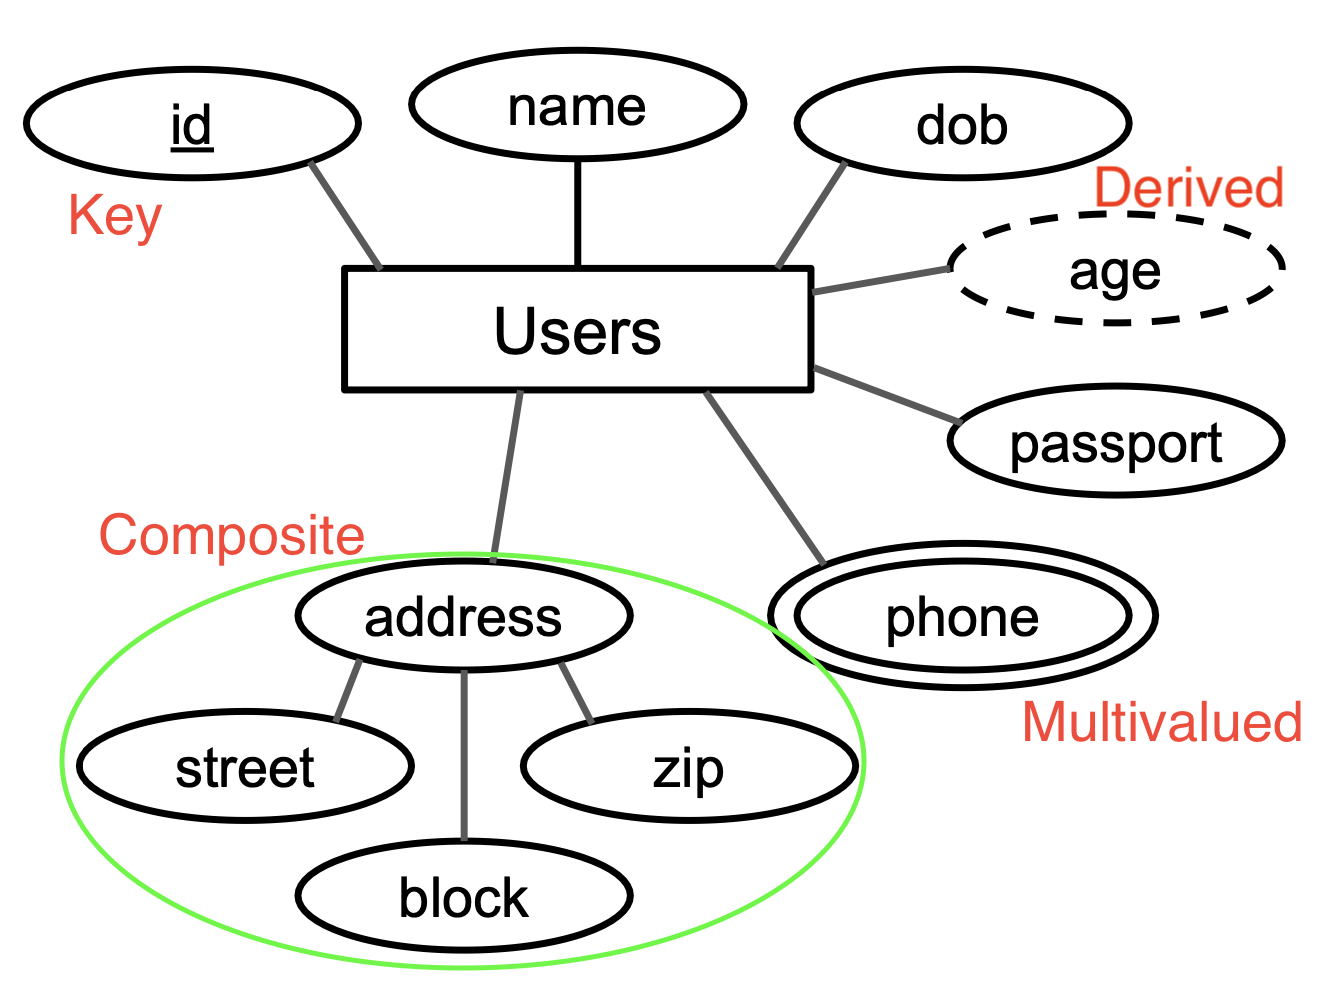
\includegraphics[width=\columnwidth]{L4/attributes}
    \end{center}
  \subsection*{Relationship} \noindent
    Association among two or more entities
    \subsubsection*{Relationship set} \noindent
      \begin{itemize}[leftmargin=*]
        \item Collection of relationships of the same type
        \item Can have their own attributes that further describe the relationship
        \item $Key(E_i)$ is the attributes of the selected key of entity set $E_i$
      \end{itemize}
      \paragraph{Role}
        \begin{itemize}[leftmargin=*]
          \item Describes an entity set's participation in a relationship
          \item Explicit role label only in case of ambiguities (e.g. same entity set participates in same relationship more than once)
        \end{itemize}
      \paragraph{Degree}
        \begin{itemize}[leftmargin=*]
          \item An $n$-ary relationship set involves $n$ entity roles, where $n$ is the degree of the relationship set
          \item Typically binary or ternary
        \end{itemize}
      \begin{minipage}{.5 \columnwidth}
        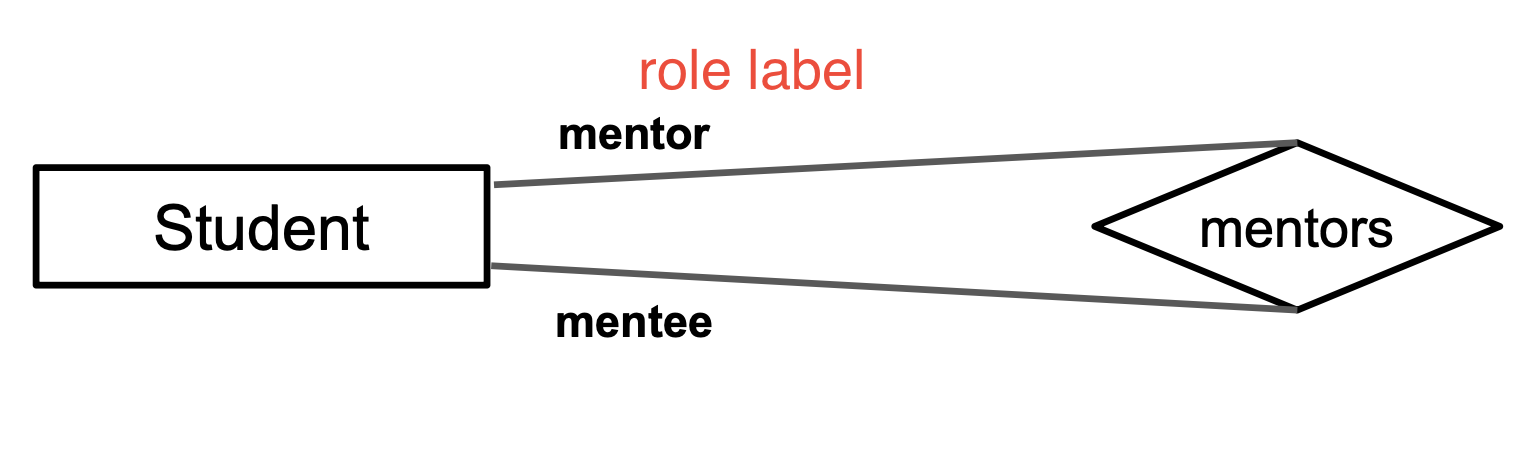
\includegraphics[width=\columnwidth]{L4/role}
      \end{minipage}
      \begin{minipage}{.475 \columnwidth}
        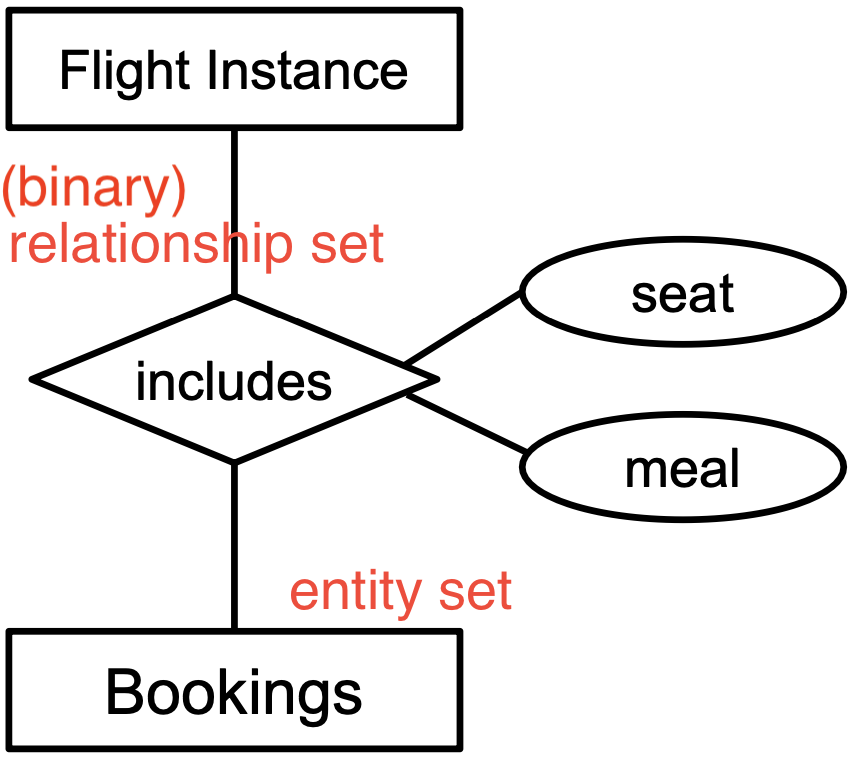
\includegraphics[width=\columnwidth]{L4/relationship-set}
      \end{minipage}
  \subsection*{Cardinality constraints}
    \begin{itemize}[leftmargin=*]
      \item \textbf{Upper bound} for entity's participation
    \end{itemize}
    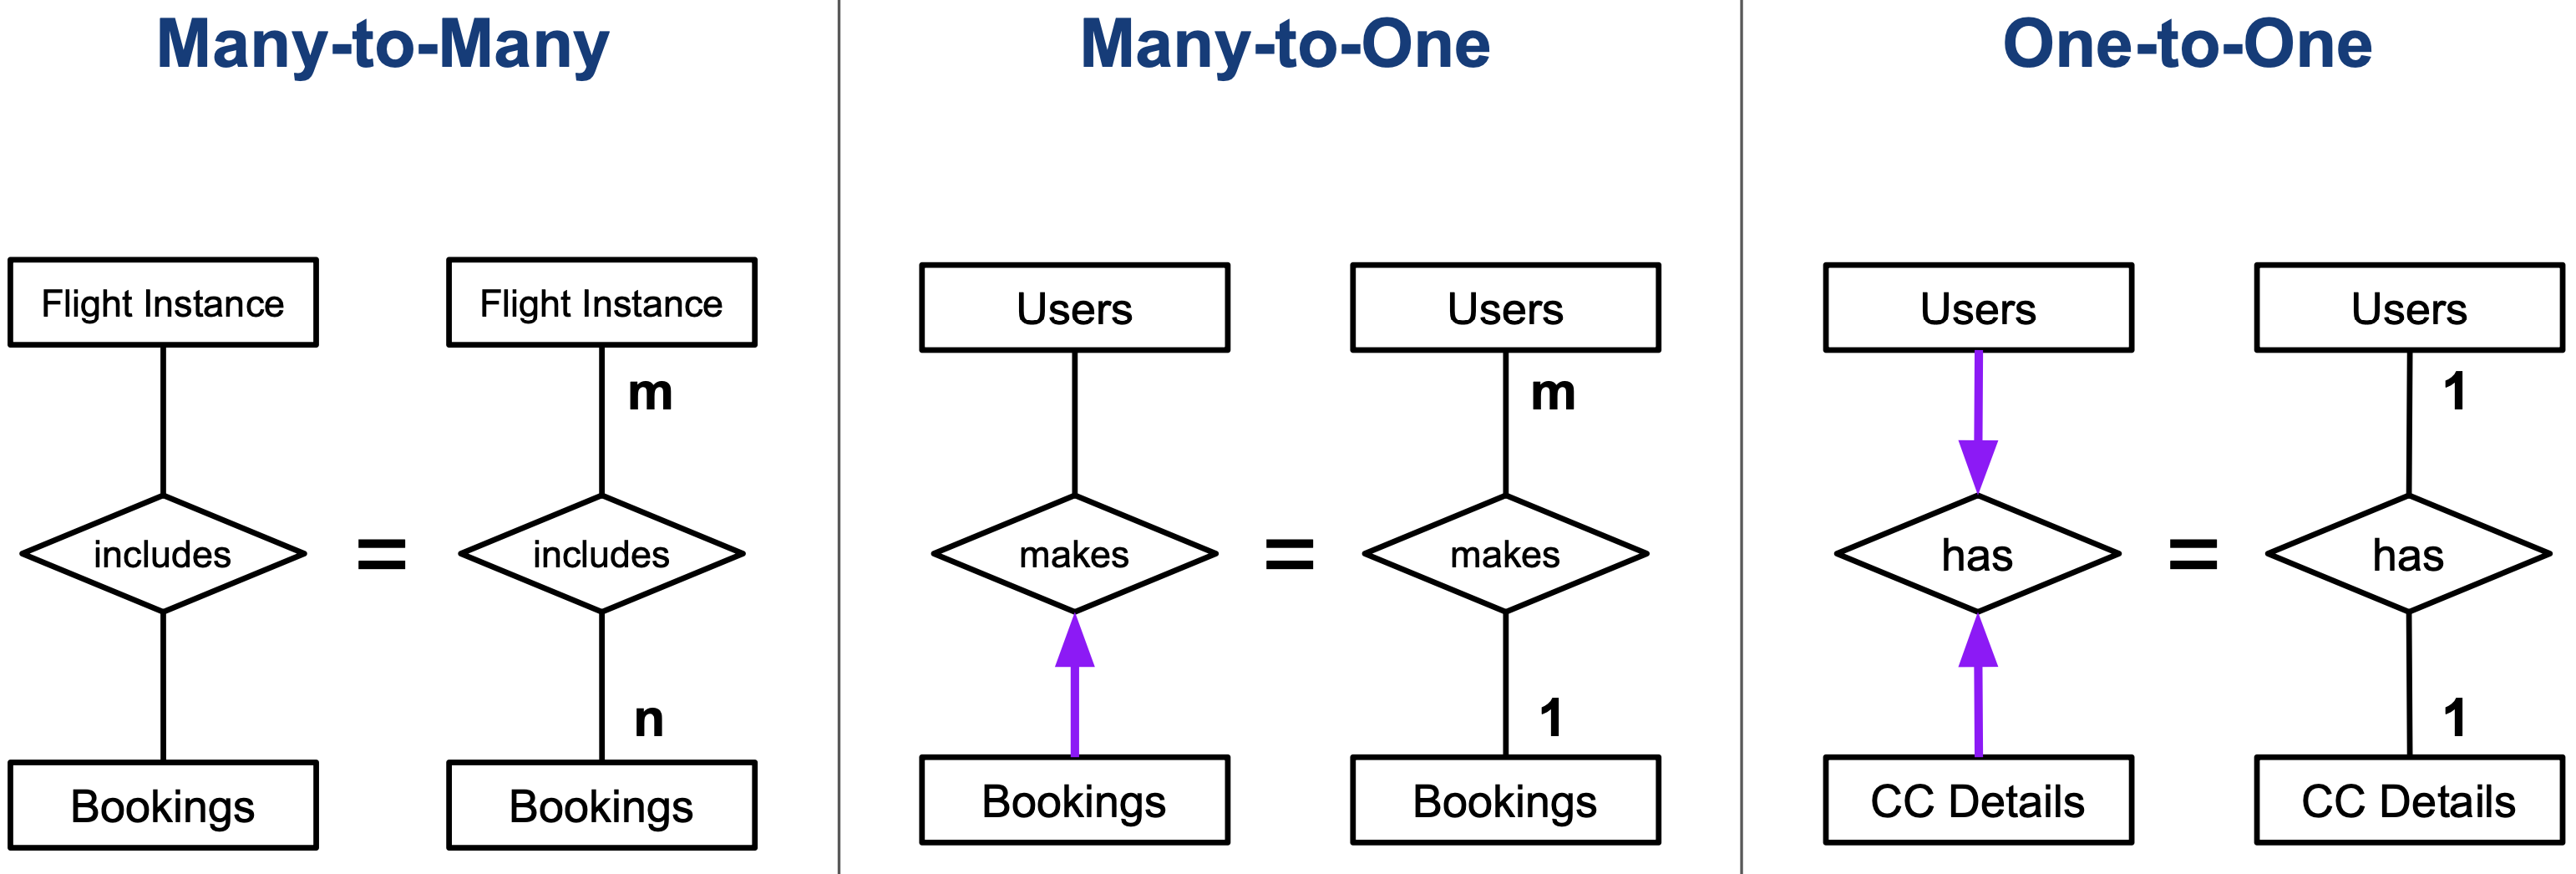
\includegraphics[width=\columnwidth]{L4/cardinality}
\end{multicols*}

\begin{multicols}{2}
  \subsection*{Participation constraints}
    \begin{itemize}[leftmargin=*]
      \item \textbf{Lower bound} for entity's participation
      \item Partial (default): participation not mandatory
      \item Total: mandatory (at least 1)
    \end{itemize}
    \begin{multicols*}{2}
      \subsubsection*{Standard}
      \begin{center}
        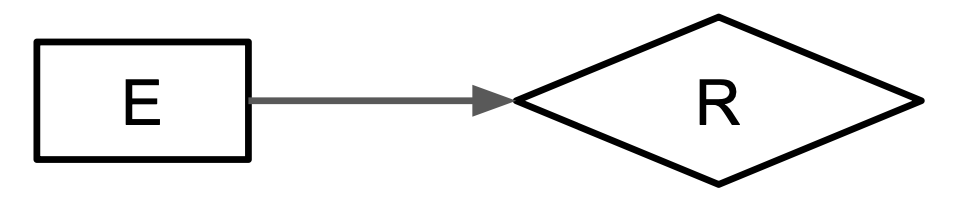
\includegraphics[width=\columnwidth]{L4/participation/at-most-one}
        At most one \\
        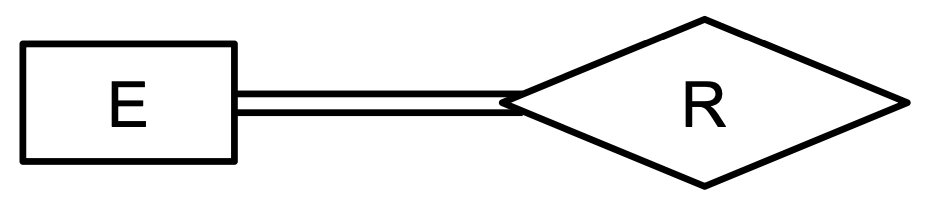
\includegraphics[width=\columnwidth]{L4/participation/at-least-one}
        At least one \\
        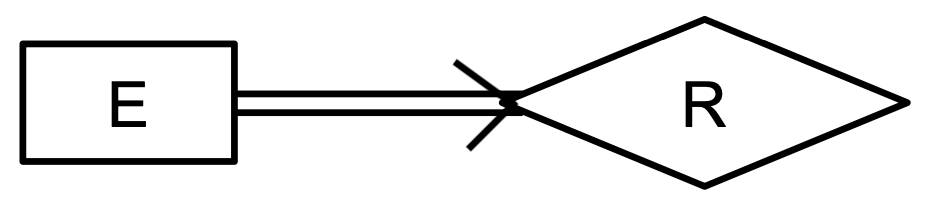
\includegraphics[width=\columnwidth]{L4/participation/exactly-one}
        Exactly one \\
      \end{center}
    \columnbreak
      \subsubsection*{Alternative} \noindent
        \begin{center}
          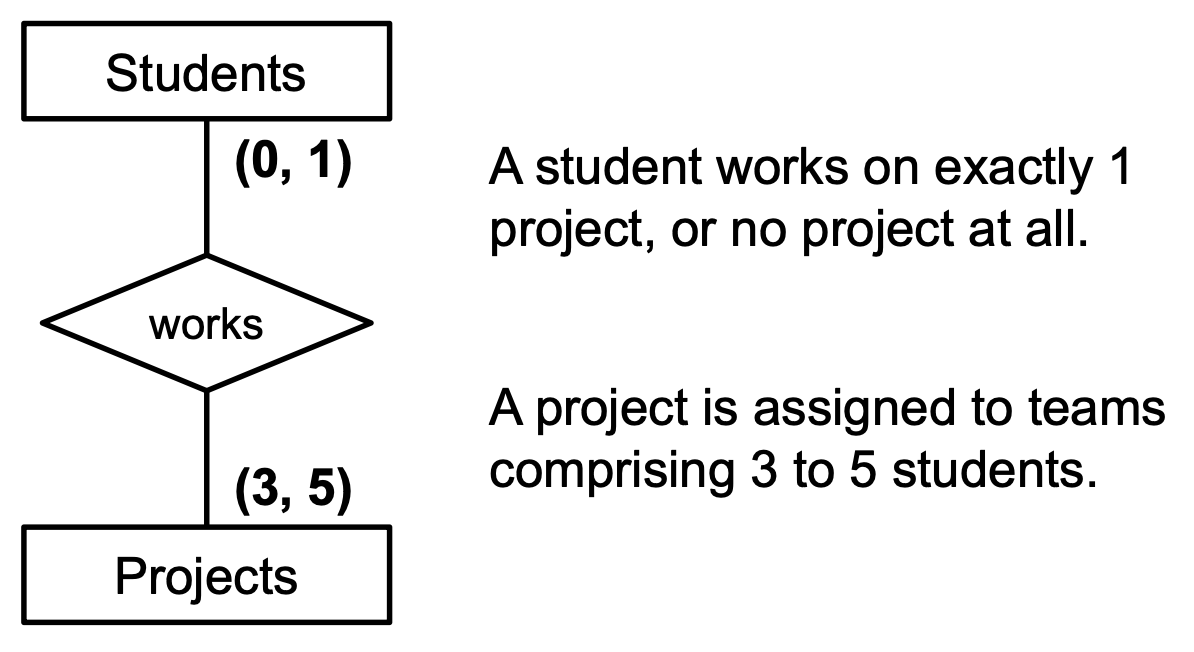
\includegraphics[width=\columnwidth]{L4/participation/min-max}
        \end{center}
    \end{multicols*}
    \subsubsection*{Implementation}
      \paragraph{Many-to-Many} Represent relationship set with a table
      \paragraph{Many-to-One}
        \begin{enumerate}[leftmargin=*]
          \item Represent relationship set between $A$ and $B$ with a table ($A_{id}$, $B_{id}$). Make the ID of the total participation entity set the primary key
          \item Combine rel. set and total participiation entity set into one table
        \end{enumerate}
      \paragraph{One-to-One}
        \begin{enumerate}[leftmargin=*]
          \item Represent relationship set between $A$ and $B$ with a table ($A_{id}$, $B_{id}$). One is unique not null, and the other is the primary key
          \item Combine relationship set and either entity set into one table
        \end{enumerate}
  \subsection*{Dependency constraints}
    \subsubsection*{Weak entity sets}
      \begin{itemize}[leftmargin=*]
        \item Entity set that does not have its own key
        \item Can only be uniquely identified by considering primary key of owner entity
        \item Existence depends on existence of owner entity
      \end{itemize}
      \paragraph{Partial key}
        \begin{itemize}[leftmargin=*]
          \item Set of attributes of weak entity set that uniquely identifies a weak entity, for a given owner entity
        \end{itemize}
      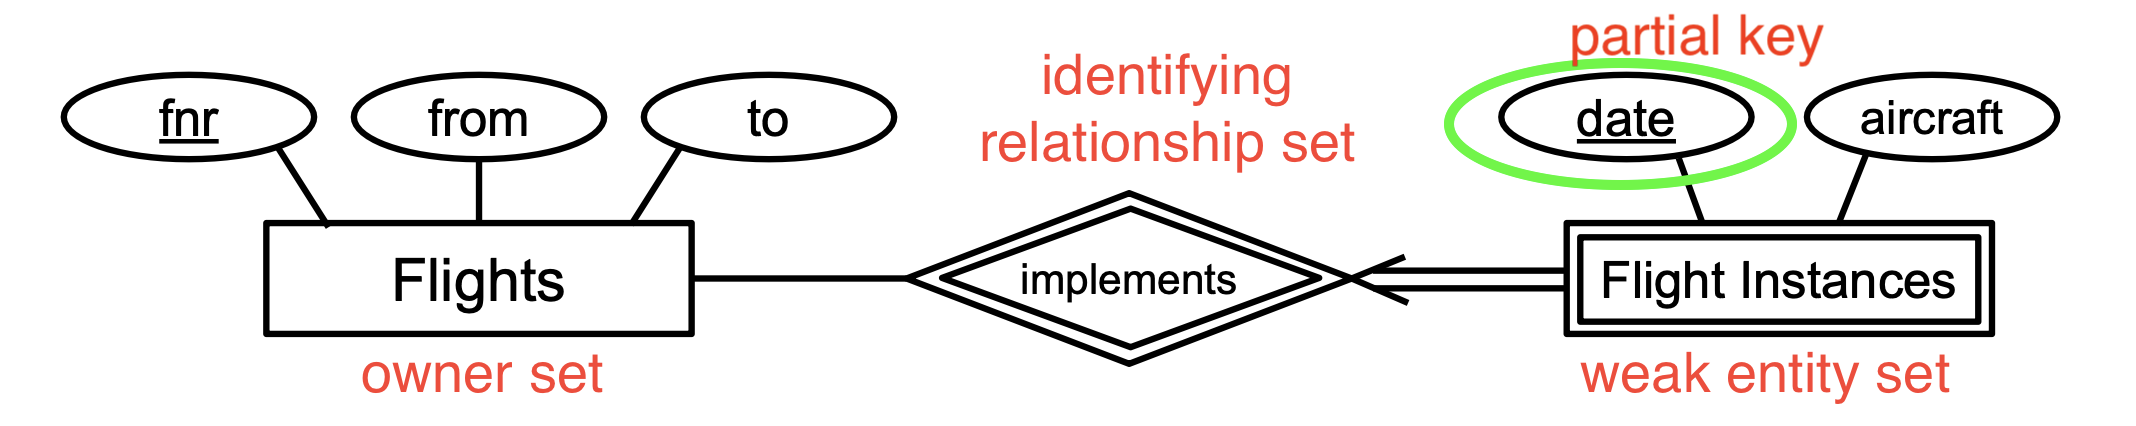
\includegraphics[width=\columnwidth]{L4/weak-entity}
      \paragraph{Requirements}
        \begin{itemize}[leftmargin=*]
          \item Many-to-one relationship from weak entity set to owner entity set
          \item Weak entity set must have total participation in identifying relationship
        \end{itemize}
  \subsection*{Relational mapping}
    \begin{itemize}[leftmargin=*]
      \item Entity set $\rightarrow$ table
      \item Composite/multivalued attributes:
        \begin{enumerate}[leftmargin=*]
          \item Convert to single-valued attributes
          \item Additional table with FK constraint
          \item Convert to a single-valued attribute (e.g. comma separated string)
        \end{enumerate}
    \end{itemize}
  \subsection*{ISA Hierarchies}
    \begin{itemize}[leftmargin=*]
      \item Used to model generalization/specialization of entity sets
    \end{itemize}
    \subsubsection*{Constraints}
      \paragraph{Overlap} Can a superclass entity belong to multiple subclasses?
      \paragraph{Covering} Does a superclass entity have to belong to a subclass?
    \begin{minipage}{.475 \columnwidth}
      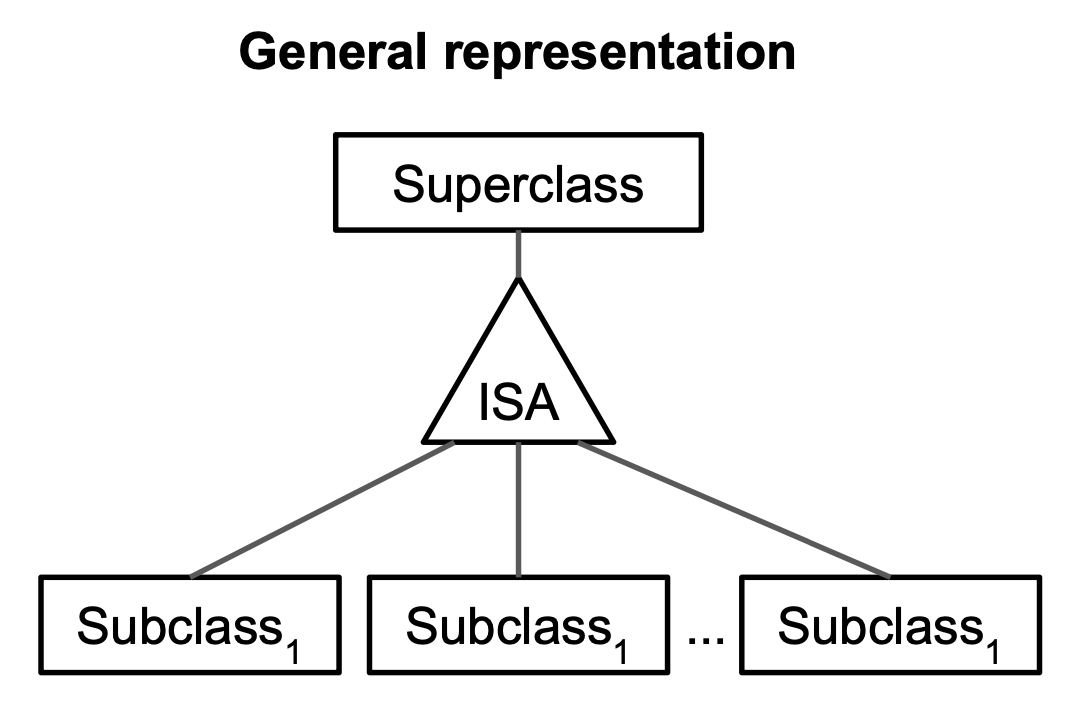
\includegraphics[width=\columnwidth]{L4/is-a}
    \end{minipage}
    \begin{minipage}{.5 \columnwidth}
      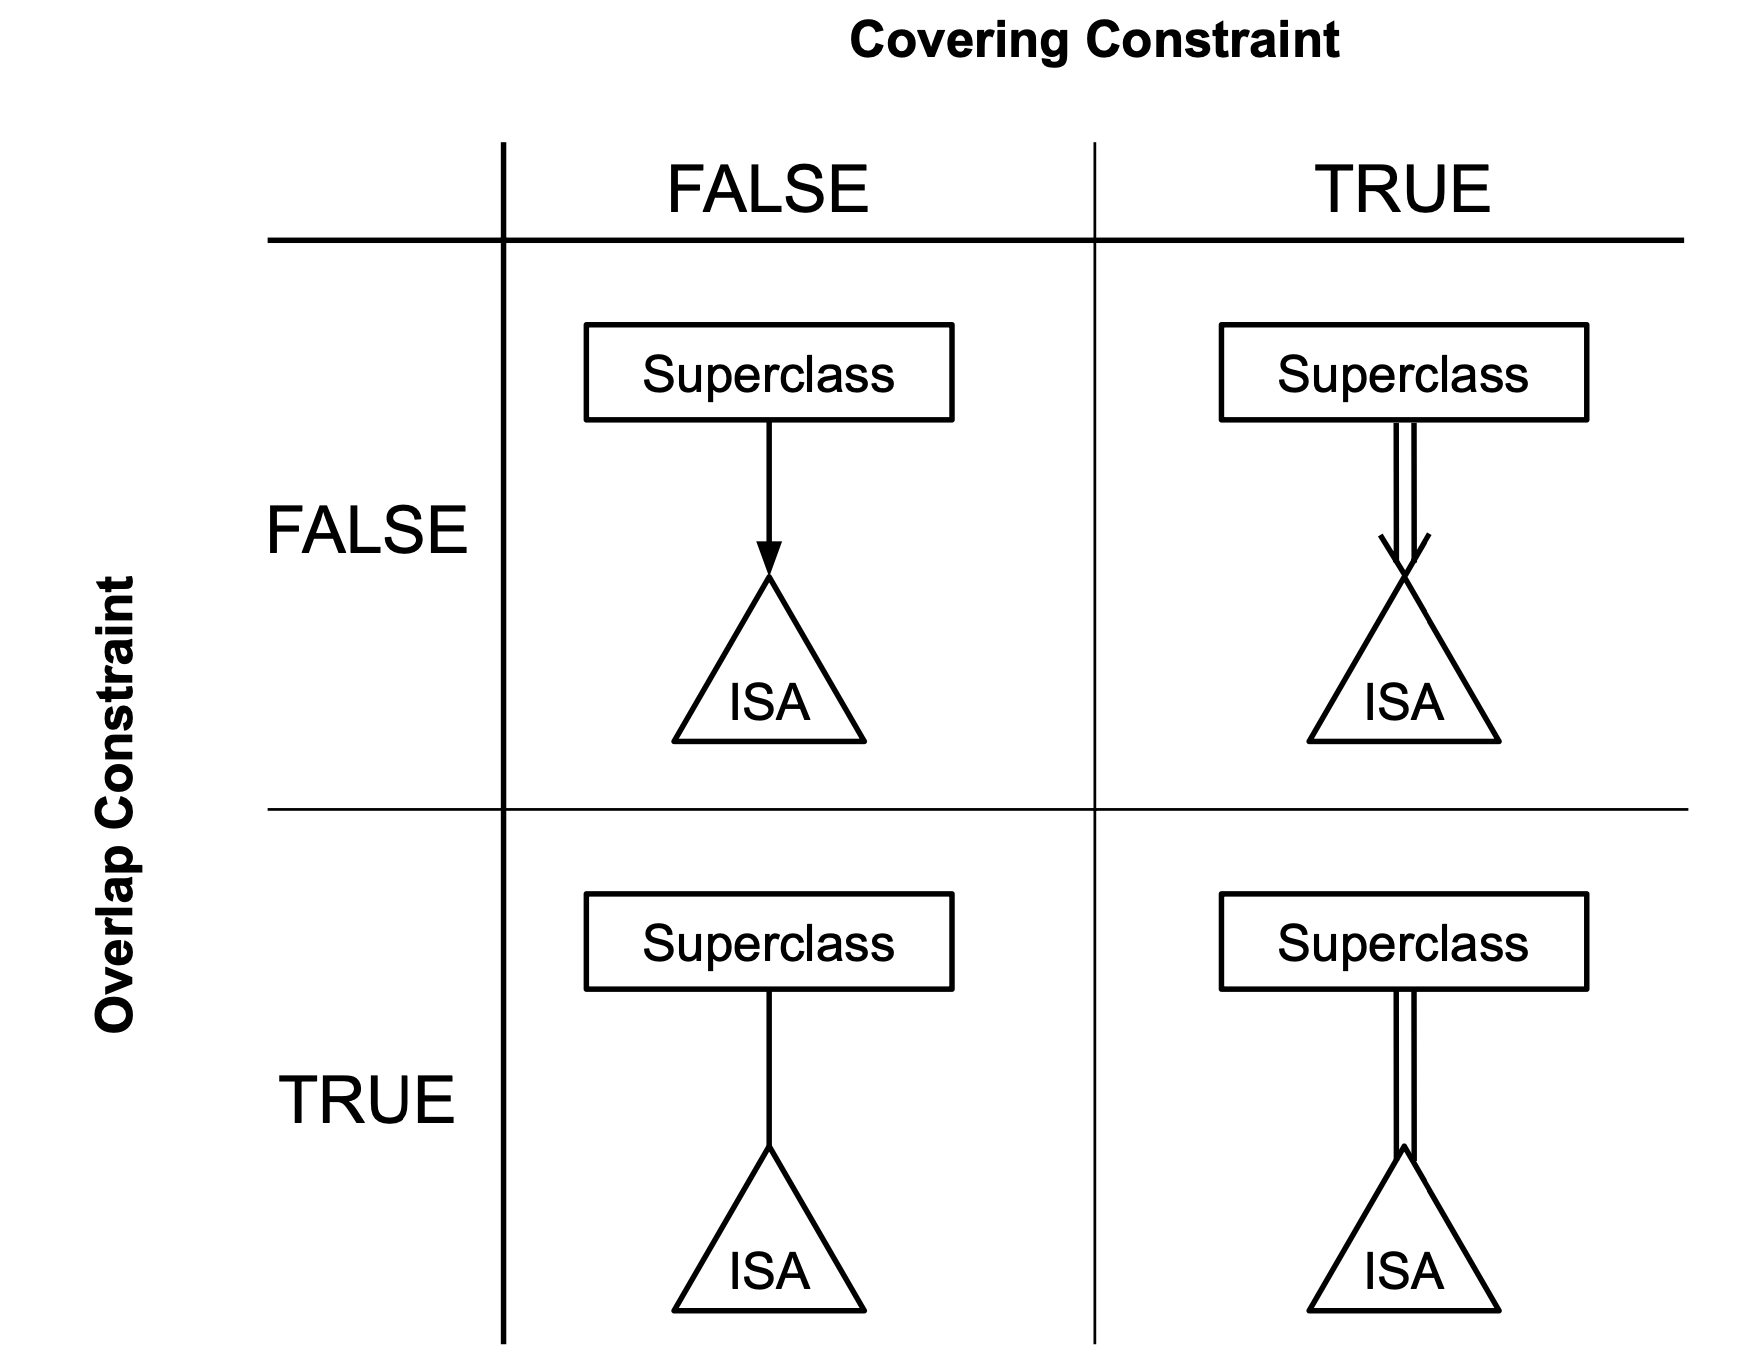
\includegraphics[width=\columnwidth]{L4/is-a-constraints}
    \end{minipage}
  \subsection*{Aggregation}
    \begin{itemize}[leftmargin=*]
      \item Abstraction that treats relationships as higher-level entities
    \end{itemize}
    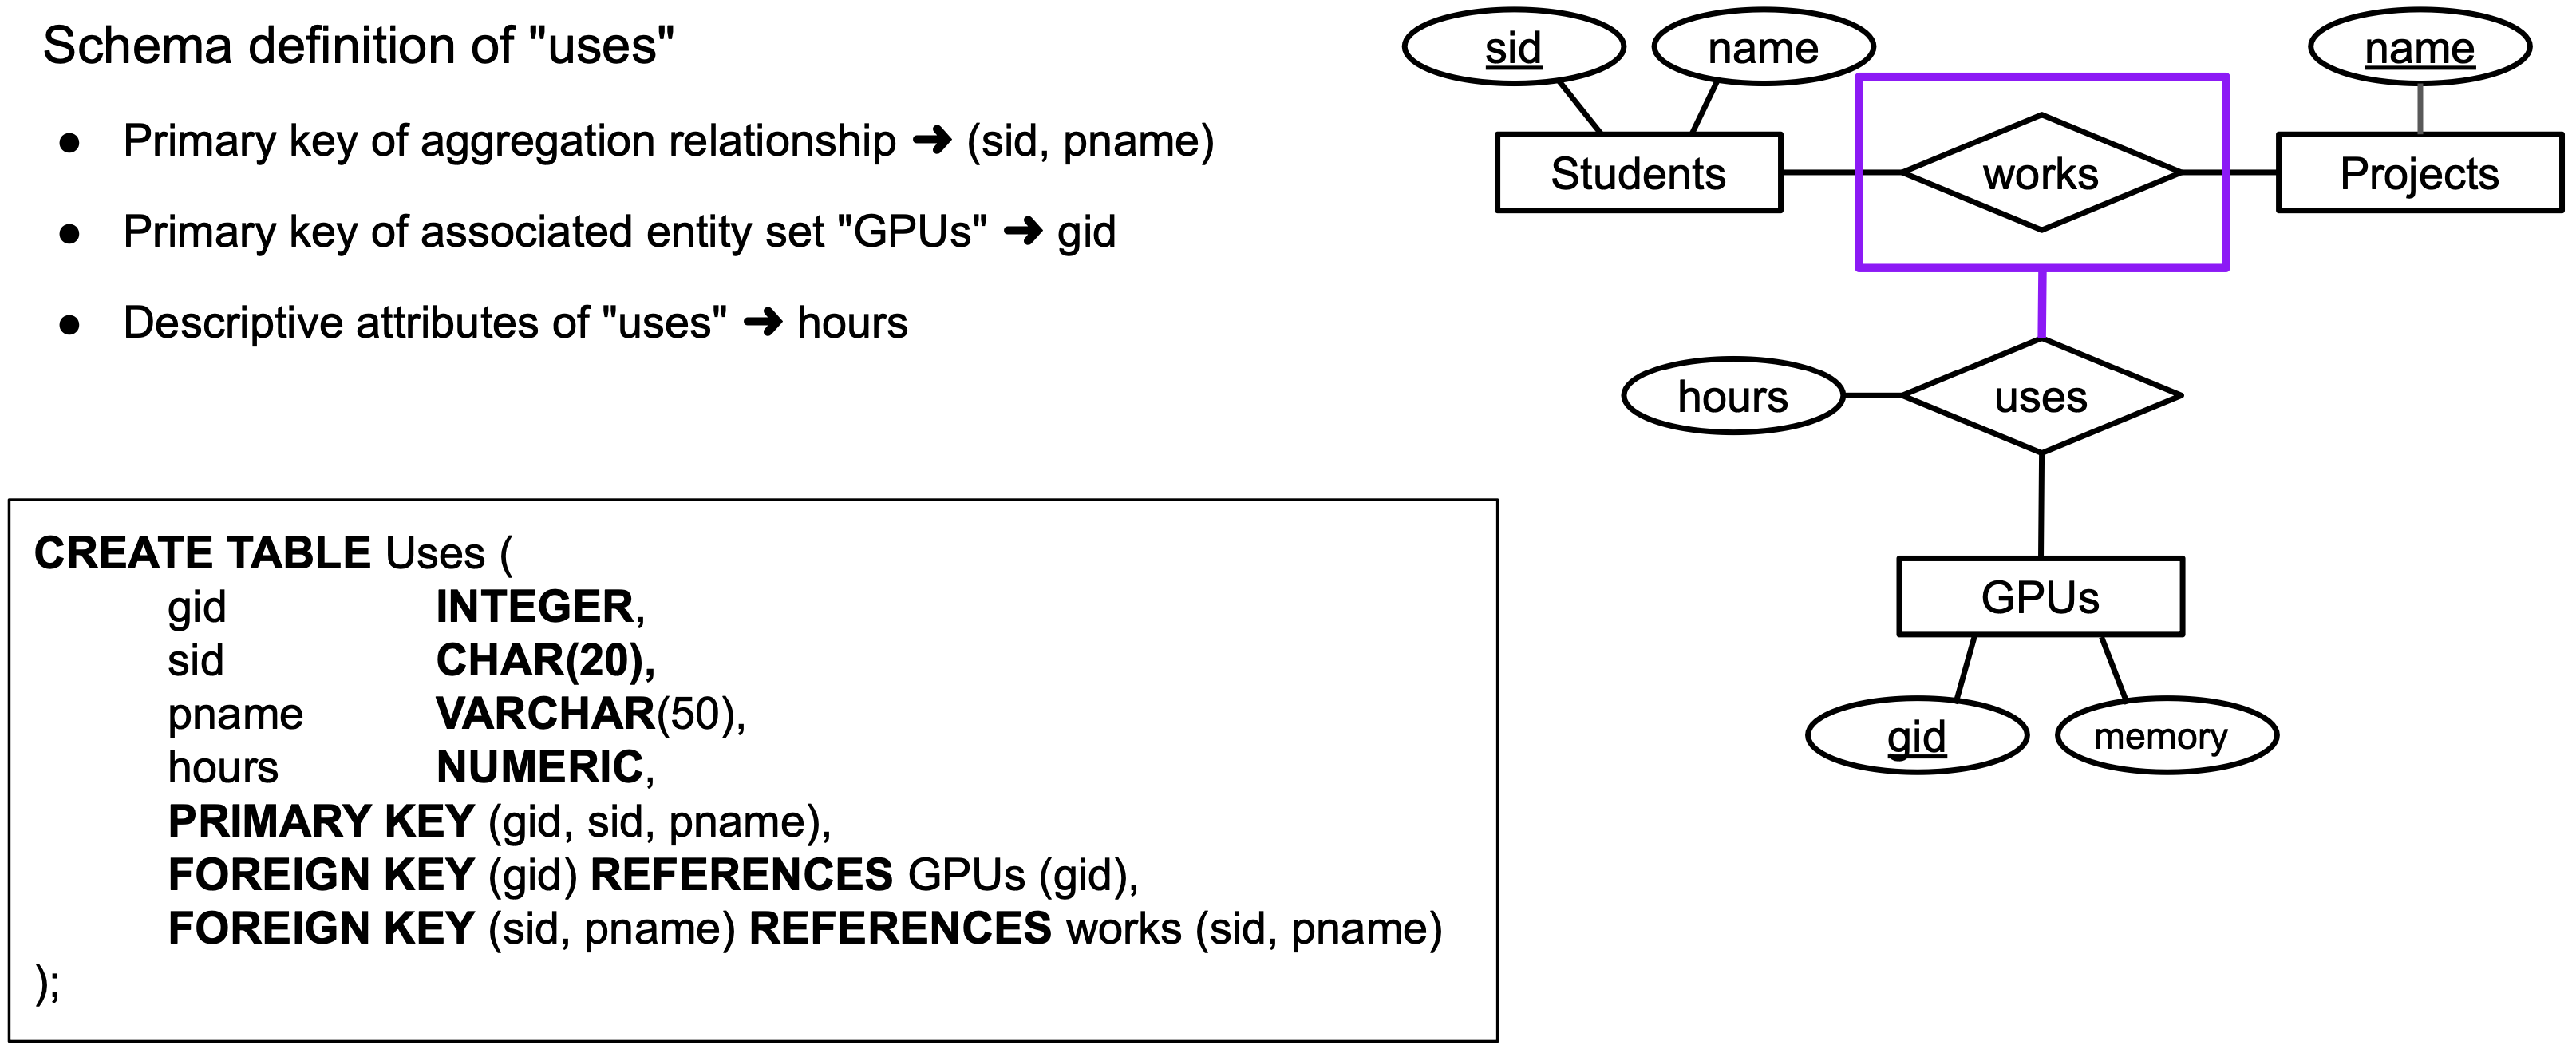
\includegraphics[width=\columnwidth]{L4/aggregation}
\section*{Functions and Procedures} \noindent
    \begin{minipage}{0.57\columnwidth}
      \begin{lstlisting}
-- Function
CREATE OR REPLACE FUNCTION <name>
(<param> <type>, ...)
RETURNS <type> AS $$
  <code>
$$ LANGUAGE <sql | plpgsql>;
-- Procedure
CREATE OR REPLACE PROCEDURE <name>
(<param> <type>, ...) AS $$
  <code>
$$ LANGUAGE <sql | plpgsql>;
      \end{lstlisting}
    \end{minipage}
    \begin{minipage}{0.40\columnwidth}
      \begin{itemize}[leftmargin=*]
        \item \ic{CREATE OR REPLACE} helps to re-declare function/procedure if already previously defined
        \item Code is enclosed within \ic{\$\$}
        \item Call a function: \ic{SELECT * FROM swap(2, 3);}
        \item Call a procedure: \ic{CALL transfer('Alice', 'Bob', 100);}
      \end{itemize}
    \end{minipage}
  \subsection*{Return types}
    \begin{center}
      \begin{tabular}{ |c|c| }
        \hline
        \textbf{Return} & \textbf{Type} \\ \hline
        Single tuple from table & \ic{<table_name>} \\ \hline
        Set of tuples from table & \ic{SET OF <table_name>} \\ \hline
        Single new tuple & \ic{RECORD} \\ \hline
        Set of new tuples & \makecell{ \ic{SET OF RECORD} or \\ \ic{TABLE(c VARCHAR, x INT)} } \\ \hline
        No return value & \makecell{ \ic{VOID}, or use \ic{PROCEDURE} \\ instead of \ic{FUNCTION} } \\ \hline
        Trigger & \ic{TRIGGER} \\ \hline
      \end{tabular}
    \end{center}
  \subsection*{Control structures}
    \begin{multicols*}{2}
      \paragraph{Variables}
        \begin{itemize}[leftmargin=*]
          \item \ic{DECLARE [<var> <type>]} (1 or more when \ic{DECLARE} keyword is present)
          \item \ic{<var> := <expr>}
        \end{itemize}
      \paragraph{Selection}
        \begin{itemize}[leftmargin=*]
          \item \ic{IF ... THEN ...} \\
                \ic{[ELSIF ... THEN ...]} \\
                \ic{[ELSE ...] END IF} \\
                (0 or more \ic{ELSIF})
        \end{itemize}
    \columnbreak
      \paragraph{Repetition}
        \begin{itemize}[leftmargin=*]
          \item \ic{LOOP ... END LOOP}, and \\
                \ic{EXIT ... WHEN ...} \\
                (conditional exit)
          \item \ic{WHILE ... LOOP ... END LOOP}
          \item \ic{FOR ... IN ... LOOP ... END LOOP}
          \item \ic{1..10} (range, inclusive)
        \end{itemize}
      \paragraph{Block}
        \begin{itemize}[leftmargin=*]
          \item \ic{BEGIN ... END}
          \item For plpgsql, code in the BEGIN-END block is in a transaction
        \end{itemize}
    \end{multicols*}
    \subsubsection*{Examples} \noindent
      Note: \ic{INOUT} specifies that the param is both an input and output param
      \begin{multicols*}{2} \noindent
        \textbf{Function}
        \begin{lstlisting}
CREATE OR REPLACE FUNCTION swap(INOUT val1 INT, INOUT val2 INT)
RETURNS RECORD AS $$
DECLARE
  temp INT;
BEGIN
  temp := val1;
  val1 := val2;
  val2 := temp;
END;
$$ LANGUAGE plpgsql;
        \end{lstlisting}
      \columnbreak
        \textbf{Procedure}
        \begin{lstlisting}
CREATE OR REPLACE PROCEDURE transfer(
 src TEXT, dst TEXT,
 amt NUMERIC
) AS $$
  UPDATE Accounts
  SET balance = balance - amt
  WHERE name = src;
  UPDATE Accounts
  SET balance = balance + amt
  WHERE name = dst;
$$ LANGUAGE sql;
        \end{lstlisting}
      \end{multicols*}
  \subsection*{Cursor}
    \begin{itemize}[leftmargin=*]
      \item Declare, Open, Fetch, Check (repeat), Close
      \item \ic{FETCH [PRIOR | FIRST | LAST | ABSOLUTE n] [FROM] <cursor> INTO <var>}
    \end{itemize}
    \begin{center}
      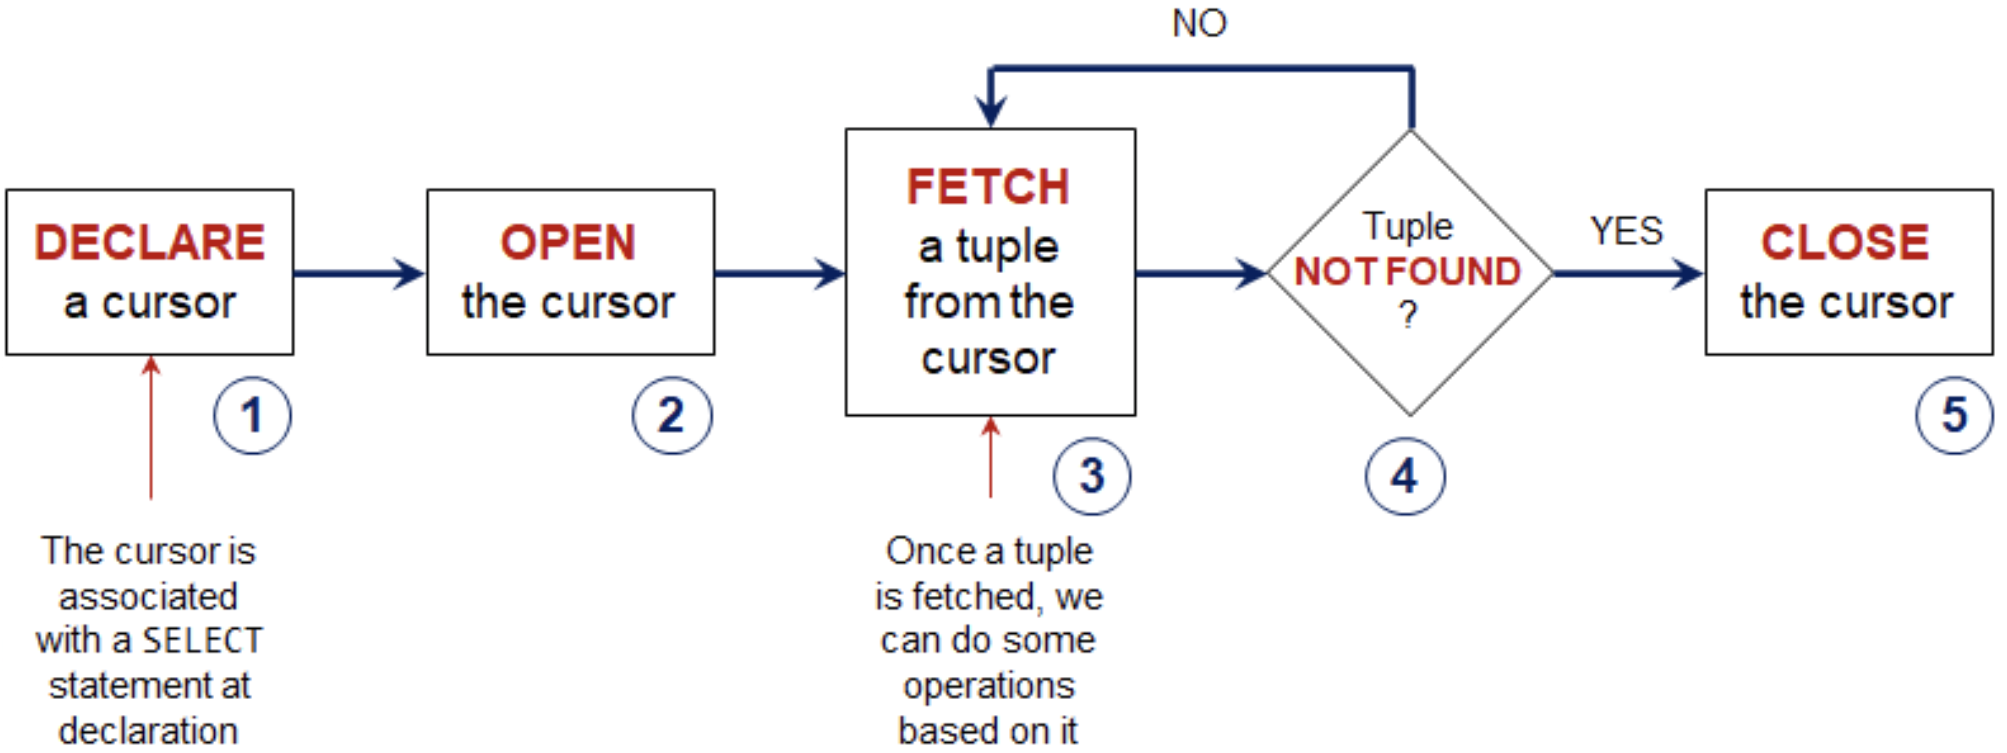
\includegraphics[width=\columnwidth]{L8/cursor_workflow}
      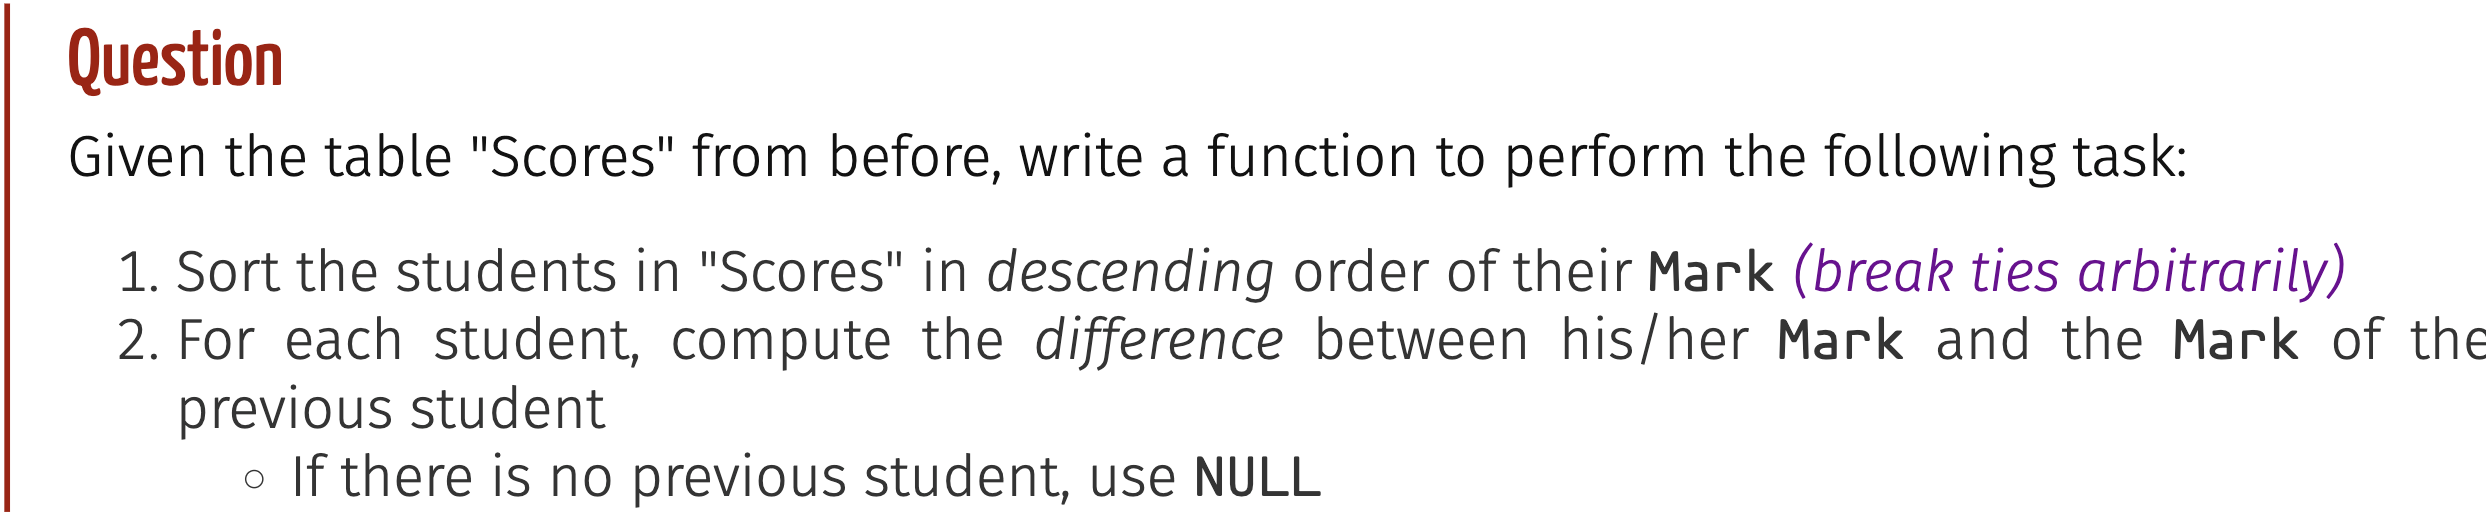
\includegraphics[width=\columnwidth]{L8/cursor_question}
      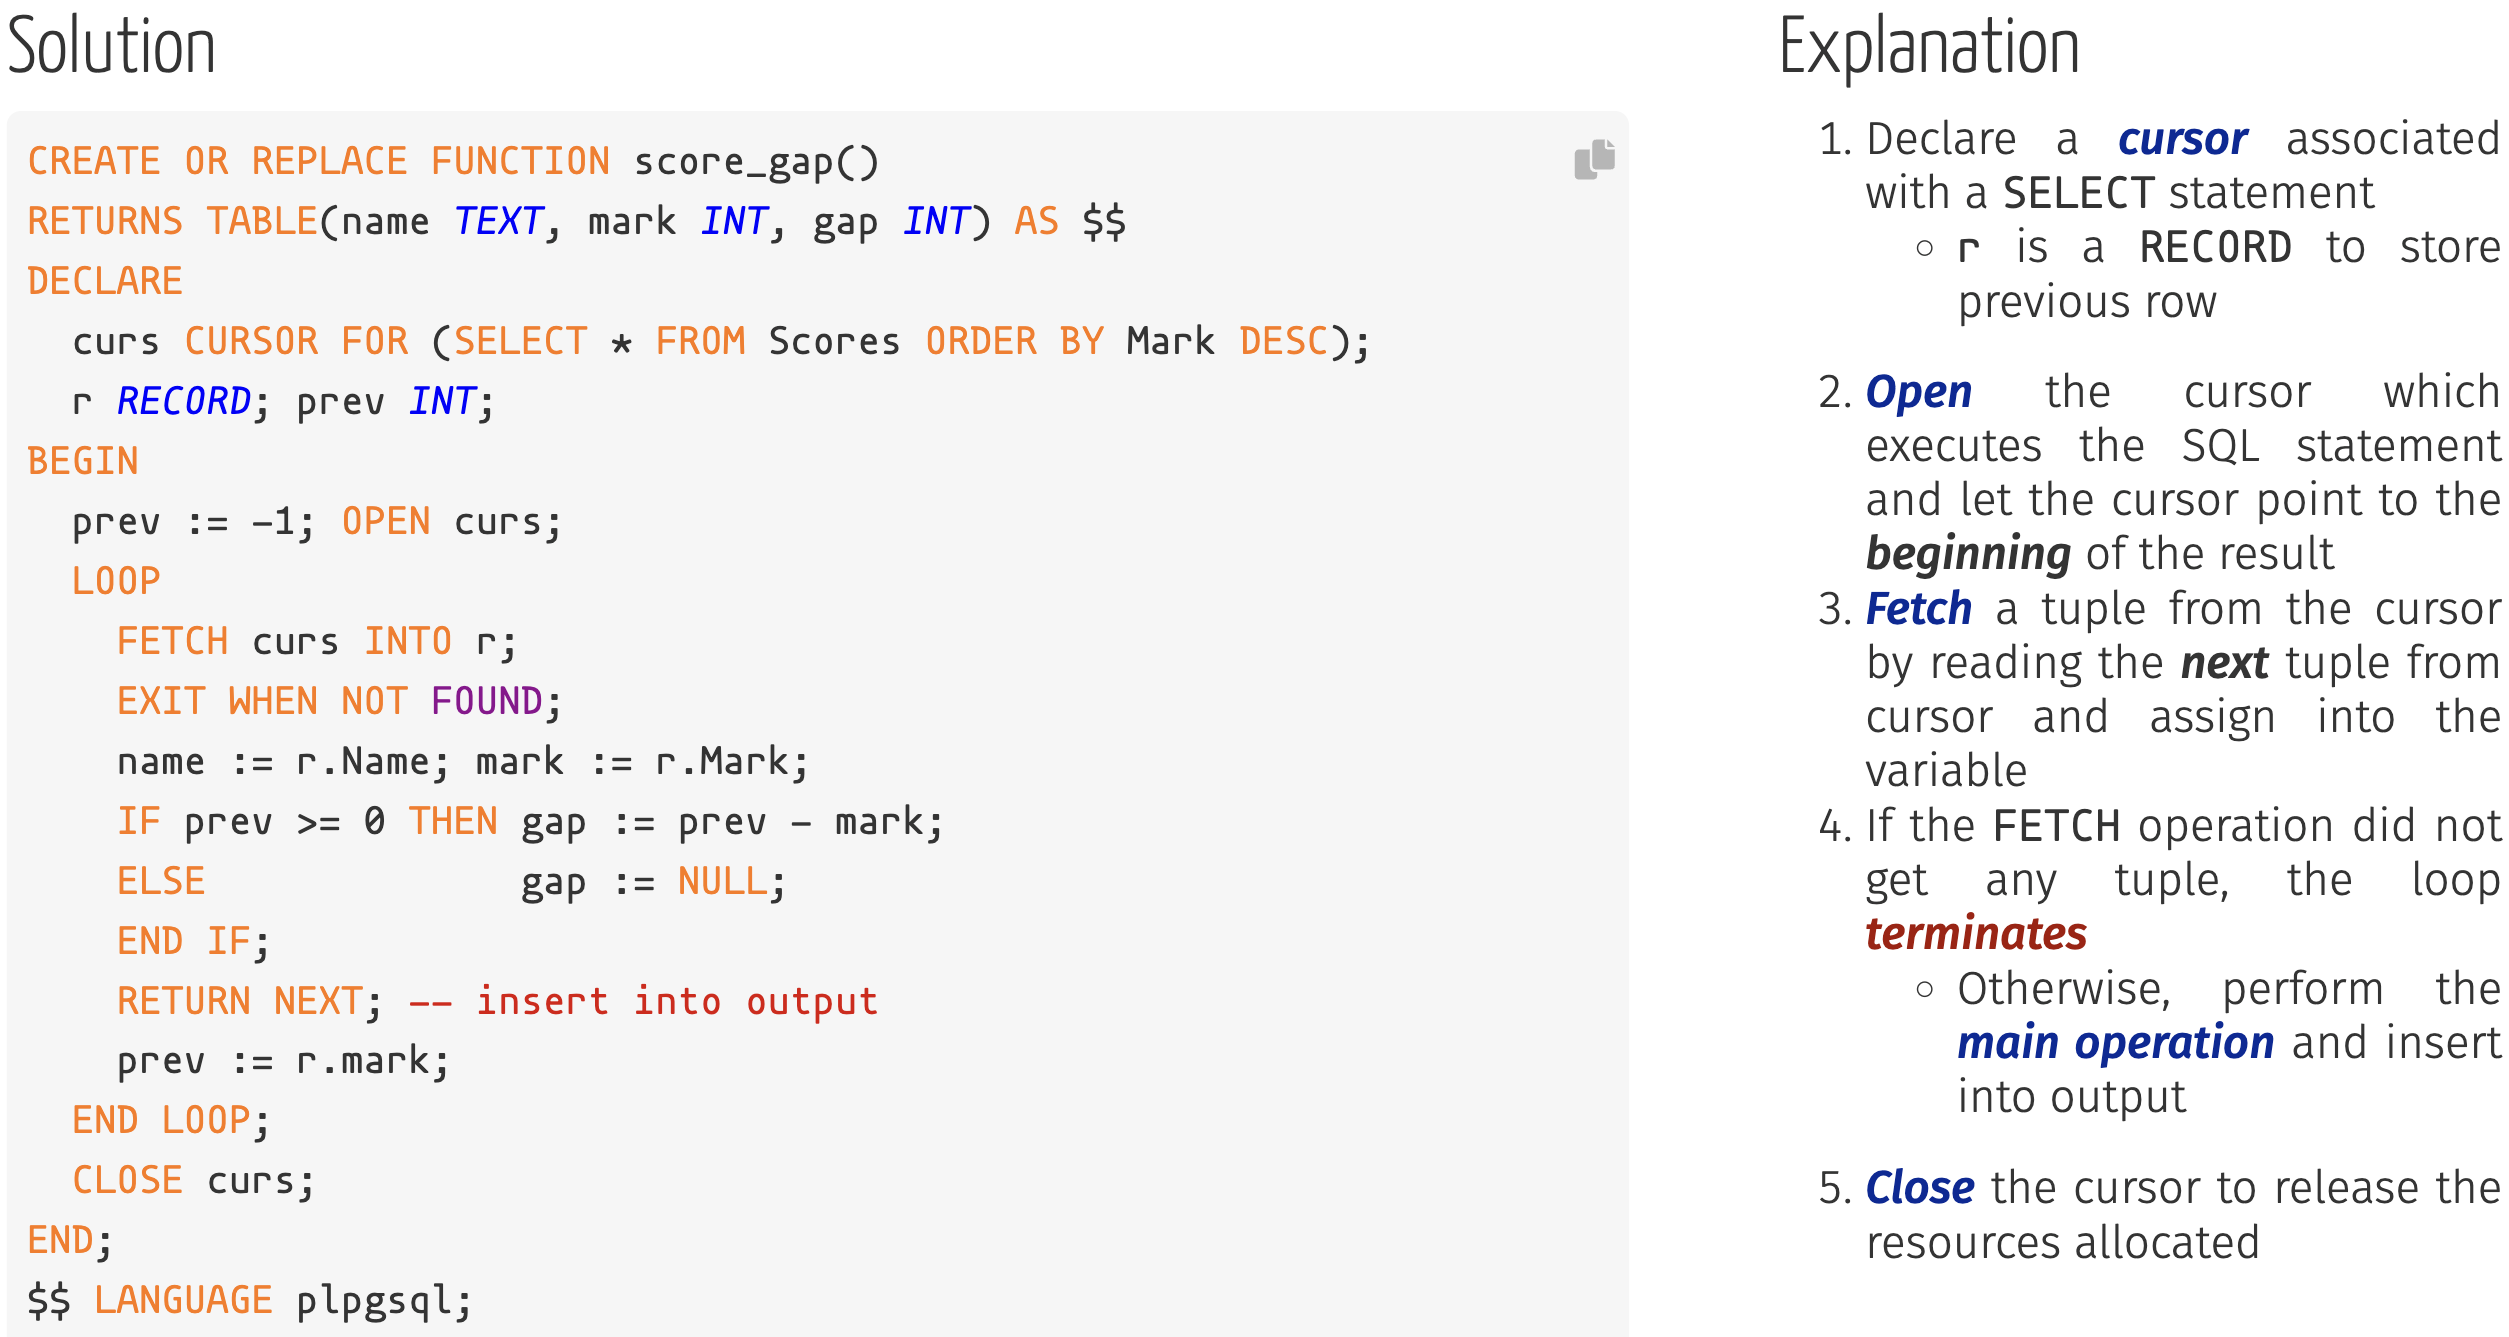
\includegraphics[width=\columnwidth]{L8/cursor_example}
    \end{center}
\section*{Triggers} \noindent
  \begin{itemize}[leftmargin=*]
    \item Note: cannot \ic{CREATE OR REPLACE TRIGGER}. Need to \ic{DROP TRIGGER}
  \end{itemize}
  \begin{minipage}{0.35\columnwidth}
    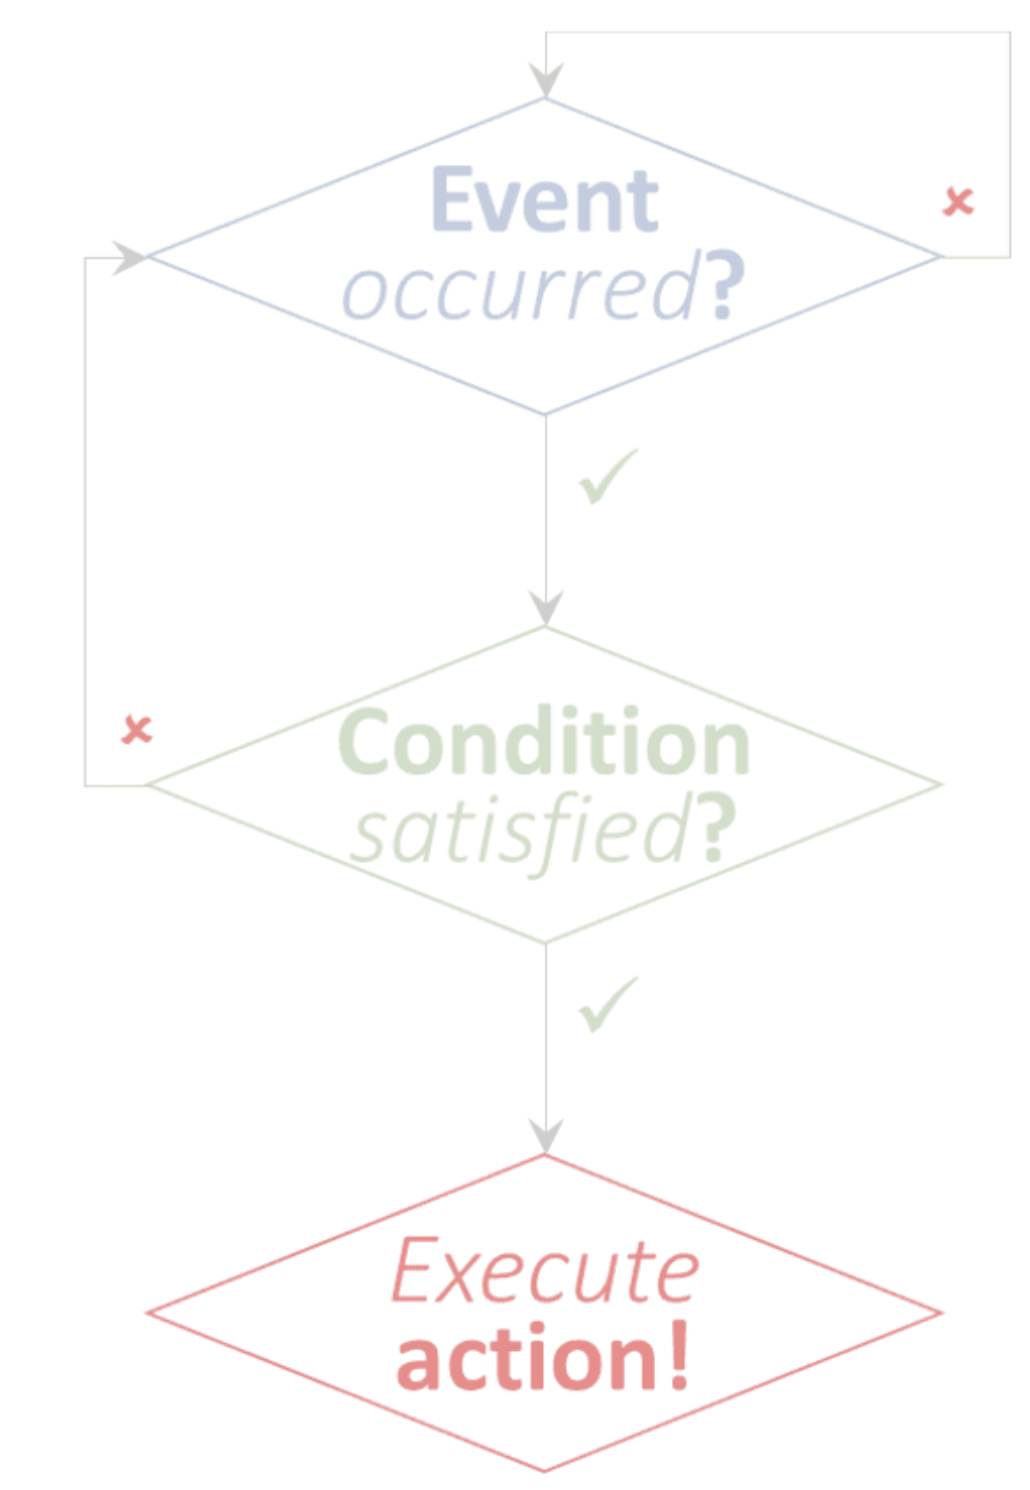
\includegraphics[width=\columnwidth]{L9/trigger_workflow}
  \end{minipage}
  \begin{minipage}{0.63\columnwidth}
    \begin{lstlisting}
-- Trigger
CREATE TRIGGER <name>
<timing> <event> ON <table>
FOR EACH <granularity>
  [ WHEN (<condition>) ]
EXECUTE FUNCTION <f_name>();
-- Trigger function
CREATE OR REPLACE FUNCTION <f_name>()
RETURNS TRIGGER AS $$
BEGIN
  <code>
END;
$$ LANGUAGE plpgsql;
    \end{lstlisting}
  \end{minipage}
  \subsection*{Trigger options}
    \begin{multicols*}{2}
      \paragraph{Events}
        \begin{itemize}[leftmargin=*]
          \item \ic{INSERT ON <table>}
          \item \ic{DELETE ON <table>}
          \item \ic{UPDATE [ OF <column> ] ON <table>}
          \item \ic{INSERT OR DELETE OR UPDATE ON <table>}
          \item Alternatively, use \ic{TG_OP} variable. Is set to \ic{'INSERT' | 'DELETE' | 'UPDATE'}
        \end{itemize}
    \columnbreak
      \paragraph{Timings}
        \begin{itemize}[leftmargin=*]
          \item \ic{AFTER/BEFORE} (after/before event)
          \item \ic{INSTEAD OF} (replaces event, only for \ic{VIEWS})
        \end{itemize}
      \paragraph{Granularity}
        \begin{itemize}[leftmargin=*]
          \item \ic{FOR EACH ROW} (for each tuple encountered)
          \item \ic{FOR EACH STATEMENT} (for each statement)
        \end{itemize}
    \end{multicols*}
    \vspace{-0.3cm}
    \subsubsection*{Effect of return value}
      \begin{itemize}[leftmargin=*]
        \item \ic{OLD} / \ic{NEW}: Modified row before / after the triggering event
      \end{itemize}
      \vspace{-0.3cm}
      \begin{center}
        \resizebox{\columnwidth}{!}{%
          \begin{tabular}{ |c|l|l| }
            \hline
            \textbf{Events + Timings} & \textbf{NULL tuple} & \textbf{Non-NULL tuple $t$} \\ \hline
            \ic{BEFORE INSERT} & No insertion & $t$ is inserted \\
            \ic{BEFORE UPDATE} & No update & $t$ is the updated tuple \\
            \ic{BEFORE DELETE} & No deletion & Deletion proceeds as normal \\ \hline
            \ic{AFTER} & No effect & No effect \\ \hline
          \end{tabular}
        }
      \end{center}
    \subsubsection*{Granularity}
      \begin{itemize}[leftmargin=*]
        \item In \ic{FOR EACH STATEMENT}, doing \ic{RETURN NULL} will not do anything
        \item Need to use \ic{RAISE EXCEPTION} to stop the operation
      \end{itemize}
    \subsubsection*{Trigger condition}
      \begin{itemize}[leftmargin=*]
        \item Use \ic{WHEN()} for conditional check whether a trigger should run
        \item e.g. \ic{WHEN (NEW.StuName = 'Adi')}
      \end{itemize}
      \paragraph{Usage} \noindent
        \vspace{-0.2cm}
        \begin{multicols*}{2}
          \begin{itemize}[leftmargin=*]
            \item No \ic{SELECT} in \ic{WHEN()}
            \item No \ic{OLD} in \ic{WHEN()} for \ic{INSERT}
          \end{itemize}
        \columnbreak
          \begin{itemize}[leftmargin=*]
            \item No \ic{NEW} in \ic{WHEN()} for \ic{DELETE}
            \item No \ic{WHEN()} for \ic{INSTEAD OF}
          \end{itemize}
        \end{multicols*}
      \vspace{-0.3cm}
  \subsection*{Deferred triggers}
    \begin{itemize}[leftmargin=*]
      \item Triggers that are checked only at the end of a transaction
      \item \ic{CONSTRAINT} + \ic{DEFERRABLE} together indicate that trigger can be deferred
      \item Only works with \ic{AFTER} and \ic{FOR EACH ROW}
      \item Default is \ic{IMMEDIATE}
    \end{itemize}
    \begin{lstlisting}
CREATE CONSTRAINT TRIGGER <name>
AFTER <event> ON <table>
FOR EACH ROW 
  [ WHEN (<condition>) ]
  [ DEFERRABLE INITIALLY [ DEFERRED | IMMEDIATE ] ]
EXECUTE FUNCTION <func_name>();
    \end{lstlisting}
  \subsection*{Multiple triggers}
    \begin{itemize}[leftmargin=*]
      \item Activation order for the same event on the same table:
    \end{itemize}
      \vspace{-0.3cm}
    \begin{multicols*}{2}
      \begin{enumerate}[leftmargin=*]
        \item \ic{BEFORE} statement-level triggers
        \item \ic{BEFORE} row-level triggers
        \item \ic{AFTER} row-level triggers
        \item \ic{AFTER} statement-level triggers
      \end{enumerate}
    \end{multicols*}
      \vspace{-0.3cm}
    \begin{itemize}[leftmargin=*]
      \item Within the same category, triggers are activated in alphabetical order
      \item If \ic{BEFORE} row-level trigger returns \ic{NULL}, then subsequent triggers on the same row are omitted
    \end{itemize}
\section*{Functional Dependencies}
  \subsection*{Basic terminology}
    \paragraph{Reading FDs}
      $X \rightarrow Y$ reads:
      \begin{hlist}
        \item $X$ (functionally) determines $Y$
        \item $Y$ is functionally dependent on $X$
        \item $X$ implies $Y$ (casual)
      \end{hlist}
    \paragraph{Instance}
      An instance $r$ (a table) of a relation $R$ satisifes the FD $\sigma: X \rightarrow Y$ with $X \subset R$ and $Y \subset R$, $\iff$ if two tuples of $r$ agree on their $X$-values, then they agree on their $Y$-values
    \paragraph{Valid instance} 
      An instance $r$ of relation $R$ is a valid instance of $R$ with $\Sigma \iff$ it satisfies $\Sigma$
    \paragraph{Violations}
      An instance $r$ of relation $R$ violates a set of FDs $\Sigma \iff$ does not satisfy $\Sigma$
    \paragraph{Holds}
      \begin{itemize}[leftmargin=*]
        \item A relation $R$ with a set of FDs $\Sigma$, $R$ with $\Sigma$, refers to the set of valid instances of $R$ wrt. to the FDs in $\Sigma$
        \item When a set of FDs $\Sigma$ holds on a relation $R$, only consider the valid instances of $R$ with $\Sigma$
      \end{itemize}
    \paragraph{Trivial} $X \rightarrow Y$ is trivial $\iff Y \subset X$
    \paragraph{Non-trivial} $X \rightarrow Y$ is non-trivial $\iff Y \not\subset X$
    \paragraph{Completely non-trivial} $X \rightarrow Y$ is completely non-trivial $\iff Y \neq \emptyset$ and $Y \cap X = \emptyset$
  \subsection*{Key terminology}
    \paragraph{Superkey} Let $S \subset R$ be a set of attributes of $R$. $S$ is a superkey of $R \iff S \rightarrow R$
    \paragraph{Candidate key} A superkey such that no proper subset is also a superkey
    \paragraph{Primary key} Chosen candidate key, or the candidate key if there is only one
    \paragraph{Prime attribute} An attribute that appears in some candidate key of $R$ with $\Sigma$. If not, then it is a non-prime attribute
  \subsection*{FD terminology}
    \paragraph{Closure} Let $\Sigma$ be a set of FDs of a relation $R$. The closure of $\Sigma$, denoted $\Sigma^+$, is the set of all FDs logically entailed by the FDs in $\Sigma$
    \paragraph{Equivalence} Two FDs are equivalent $\iff$ have the same closure
    \paragraph{Cover} $\Sigma_1$ is a cover of $\Sigma_2$ (and vice versa) $\iff$ their closure are equivalent
    \paragraph{Closure of a set of attributes} Let $\Sigma$ be a set of FDs of a relation $R$. The closure of a set of attributes $S \subset R$, denoted $S^+$, is the set of all attributes that are functionally dependent on $S$ (i.e. what $S$ implies)
      \\
      \[ S^+ = \{ A \in R \;\vert\; \exists (S \rightarrow \{A\}) \in \Sigma^+ \} \]
\end{multicols}

\begin{multicols*}{3}
  \subsection*{Computing attribute closures}
    \begin{itemize}[leftmargin=*]
      \item Check if any attribute doesn't appear in the RHS of any FD. These attributes must appear in the key
      \item Compute attribute closure starting with singular attributes. Then compute for 2 elements, 3 elements and so on.
      \item Note all \uline{candidate keys} in the process
      \item If current set of attributes is a superset of some previously seen, candidate key, can skip
    \end{itemize}
  \subsection*{Armstrong axioms}
      \paragraph{Reflexivity}
        \( \forall X, Y \subset R \; \Big( (Y \subset X) \Rightarrow (X \rightarrow Y) \Big) \)
      \paragraph{Augmentation}
        \[ \forall X, Y, Z \subset R \; \Big( (X \rightarrow Y) \Rightarrow (X \cup Z \rightarrow Y \cup Z) \Big) \]
      \paragraph{Transitivity}
        \[ \forall X, Y, Z \subset R \; \Big( (X \rightarrow Y) \land (Y \rightarrow Z) \Rightarrow (X \rightarrow Z) \Big) \]
    \subsubsection*{Remarks} \noindent
      \begin{itemize}[leftmargin=*]
        \item \textbf{Sound}: The rule only generates elements of $\Sigma^+$ when applied to $\Sigma$
        \item \textbf{Complete}: The rule(s) generate(s) all elements of $\Sigma^+$ when applied to $\Sigma$
        \item The three inference rules are (individually) sound
        \item The Armstrong axioms are (together) sound and complete
      \end{itemize}
  \subsection*{Additional rules} \noindent
    Must be derived during exam
    \subsubsection*{Weak augmentation} \noindent
      If $X \rightarrow Y$, then $X \cup Z \rightarrow Y$
      \paragraph{Proof}
        \begin{enumerate}[leftmargin=*]
          \item $X \rightarrow Y$ (given)
          \item We know that $X \subset X \cup Z$
          \item $X \cup Z \rightarrow X$ (reflexivity)
          \item $X \cup Z \rightarrow Y$ (trans. of 3 and 1)
        \end{enumerate}
    \subsubsection*{Union} \noindent
      If $X \rightarrow Y$ and $X \rightarrow Z$, then $X \rightarrow Y \cup Z$
      \paragraph{Proof}
        \begin{enumerate}[leftmargin=*]
          \item $X \rightarrow Y$ (given)
          \item $X \rightarrow Z$ (given)
          \item $X \rightarrow X \cup Z$ (aug. 2 and $X$)
          \item $X \cup Z \rightarrow Y \cup Z$ (aug. 1 and $Z$)
          \item $X \rightarrow Y \cup Z$ (trans. of 3 and 4)
        \end{enumerate}
    \subsubsection*{Decomposition} \noindent
      If $X \rightarrow Y \cup Z$, then $X \rightarrow Y$ and $X \rightarrow Z$
      \paragraph{Proof}
        \begin{enumerate}[leftmargin=*]
          \item $X \rightarrow Y \cup Z$ (given)
          \item $Y \cup Z \rightarrow Y$ (reflexivity)
          \item $X \rightarrow Y$ (trans. of 1 and 2)
        \end{enumerate}
    \subsubsection*{Composition} \noindent
      If $X \rightarrow Y$ and $A \rightarrow B$, then $X \cup A \rightarrow Y \cup B$
      \paragraph{Proof}
        \begin{enumerate}[leftmargin=*]
          \item $X \rightarrow Y$ (given)
          \item $A \rightarrow B$ (given)
          \item $X \cup A \rightarrow Y \cup A$ (aug. 1 and $A$)
          \item $X \cup A \rightarrow Y$ (decomp. of 3)
          \item $X \cup A \rightarrow X \cup B$ (aug. 2 and $X$)
          \item $X \cup A \rightarrow B$ (decomp. of 5)
          \item $X \cup A \rightarrow Y \cup B$ (union 4 and 6)
        \end{enumerate}
    \subsubsection*{Pseudo-transitivity} \noindent
      If $X \rightarrow Y$ and $Y \cup Z \rightarrow W$, then $X \cup Z \rightarrow W$
      \paragraph{Proof}
        \begin{enumerate}[leftmargin=*]
          \item $X \rightarrow Y$ (given)
          \item $Y \cup Z \rightarrow W$ (given)
          \item $X \cup Z \rightarrow Y \cup Z$ (aug. of 1 and $Z$)
          \item $X \cup Z \rightarrow W$ (trans. of 3 and 2)
        \end{enumerate}
  \subsection*{Minimal cover}
    \subsubsection*{Definition} \noindent
      A set $\Sigma$ of FDs is minimal if and only if
      \begin{itemize}[leftmargin=*]
        \item RHS of each FD in $\Sigma$ is minimal, i.e. each FD is of the form $X \rightarrow \{A\}$
        \item LHS of each FD in $\Sigma$ is minimal, i.e. for every FD in $\Sigma$ of the form $X \rightarrow \{A\}$, there is no FD $Y \rightarrow \{A\}$ such that $Y \subset X$
        \item The set is minimal, i.e. no FD in $\Sigma$ can be derived from other FDs in $\Sigma$
      \end{itemize}
    \subsubsection*{Misc}
      \begin{itemize}[leftmargin=*]
        \item A minimal cover of a set of FDs $\Sigma$ is a set of FDs $\Sigma'$ that is both minimal and equivalent to $\Sigma$
        \item Every set of FDs has a minimal cover
      \end{itemize}
    \subsubsection*{Algorithm}
      \begin{enumerate}[leftmargin=*]
        \item Simplify RHS of every FD (by splitting FDs so that RHS of each FD is a singleton)
        \item Simplify LHS of every FD (for each FD, if a subset of LHS can imply RHS, then replace LHS with the subset)
        \item Remove redundant FDs (for each FD, start from LHS. if this FD can be derived using only other FDs, then remove it)
        \item (If \uline{compact cover} is desired) Combine FDs with same LHS
      \end{enumerate}
    \subsubsection*{Reachability}
      \begin{itemize}[leftmargin=*]
        \item The algorithm always finds a minimal cover
        \item Some minimal covers may be unreachable
        \item To reach all minimal covers, the algorithm needs to start from $\Sigma^+$
      \end{itemize}
  \subsection*{Anomalies} \noindent
    \vspace{-0.5cm}
    \begin{center}
      \resizebox{\hsize}{!}{%
        \begin{tabular}{ |c|c|c|c|c|c| }
          \hline
          \textbf{userid} & \textbf{domain} & \textbf{department} & \textbf{faculty} & \textbf{language} \\ \hline
          tanh & comp.sut.edu & computer science & computing & JavaScript \\ \hline
          tanh & comp.sut.edu & computer science & computing & Python \\ \hline
          ami & med.sut.edu & pharmacy & medicine & R \\ \hline
        \end{tabular}
      }
    \end{center}
    \begin{itemize}[leftmargin=*]
      \item Department $\rightarrow$ faculty is a FD in this example
      \item \textbf{Redundant storage}: The faculty of a department is repeated for every student of the department, and every time the student is proficient in a language
      \item \textbf{Update anomaly}: When 2 rows of the table have the same value for the column \ic{department} but different values for the column \ic{faculty}, violating the FD
      \item \textbf{Deletion anomaly}: If we delete the last row, we may forget that we have a department of pharmacy, and a faculty of medicine
      \item \textbf{Insertion anomaly}: We cannot record that the department of social science exists and the faculty of liberal arts exists, because there is no student from this department or this faculty
    \end{itemize}
    \subsubsection*{Solution}
      \begin{itemize}[leftmargin=*]
        \item In all cases, the solution is to remove faculty from the original table, and create a new table with department and faculty
        \item In the case of the \uline{update anomaly}, to enforce the FD, we also need to make department the primary key of the new table
      \end{itemize}
  \subsection*{Normalization}
    \subsubsection*{Normal forms}
      \begin{itemize}[leftmargin=*]
        \item Recognize designs that enforce FDs through main SQL constraints (PK, unique, not null, FK)
        \item Protect data against anomalies
      \end{itemize}
    \subsubsection*{Normalization} \noindent
      Transform (decompose) a poor design into one that enforces FDs by means of the main SQL constraints
  \subsection*{Boyce-Codd Normal Form} \noindent
    A relation $R$ with a set of FDs $\Sigma$ is in BCNF $\iff$ for every FD $X \rightarrow \{A\} \in \Sigma^+$,
    \begin{itemize}[leftmargin=*]
      \item either $X \rightarrow \{A\}$ is trivial, or
      \item $X$ is a superkey
    \end{itemize}
    \subsubsection*{Check if decomp. set of relations is in BCNF}
      \begin{enumerate}[leftmargin=*]
        \item Compute attribute closures of the original set, and project FDs to each relation $R_i$
        \item If some $R_i$ is not in BCNF, then FALSE. Else TRUE
      \end{enumerate}
  \subsection*{Decomposition}
    \subsubsection*{Terminology}
      \paragraph{Decomposition} A decomposition of table $R$ is a set of tables $\{R_1, R_2, \cdots, R_n\}$ such that $R = R_1 \cup \cdots \cup R_n$
      \paragraph{Binary decomposition} Decomp with $n=2$
      \paragraph{Lossless-join definitions}
        \begin{itemize}[leftmargin=*]
          \item A binary decomp is lossless-join $\iff$ full outer natural join of its two fragments equal the initial table. Otherwise it is lossy
          \item A \uline{binary decomp} of $R$ into $R_1$ and $R_2$ is lossless-join if $R = R_1 \cup R_2$ and either $R_1 \cap R_2 \rightarrow R_1$ or $R_1 \cap R_2 \rightarrow R_2$
          \item A \uline{decomp} is lossless-join if there exists a sequence of binary lossless-join decomp that generates that decomp
        \end{itemize}
      \paragraph{Projected FDs} A set $\Sigma$ of projected FDs on $R'$, from $R$ with $\Sigma$ where $R' \subset R$, is the set of FDs equivalent to the set of FDs $X \rightarrow Y$ in $\Sigma^+$ such that $X \subset R'$ and $Y \subset R'$
      \paragraph{Dependency preserving} A decomp of $R$ with $\Sigma$ into $R_1, R_2, \cdots, R_n$ with respective projected FDs $\Sigma_1, \Sigma_2, \cdots, \Sigma_n$ is dependency preserving $\iff \Sigma^+ = (\Sigma_1 \cup \cdots \cup \Sigma_n)^+$
    \subsubsection*{Check lossless-join}
      \begin{enumerate}[leftmargin=*]
        \item Compute attribute closures of the original set
        \item For some pair $(R_i, R_j), i \neq j$,
          \begin{itemize}[leftmargin=*]
            \item Check that $R_i \cap R_j \rightarrow R_i$ or $R_i \cap R_j \rightarrow R_j$
            \item If yes, then replace $R_i, R_j$ with $R_i \cup R_j$ and repeat Step 2-3.
            \item If no, then try next pair
          \end{itemize}
        \item If there was a sequence of unions that resulted in a single relation that has all attributes, then TRUE. Else FALSE
      \end{enumerate}
    \subsubsection*{Check dependency-preserving}
      \begin{enumerate}[leftmargin=*]
        \item Let $R$ be the original set of relations. Can replace $R$ with minimal cover if found. Let $Y$ be the union of projected FDs to each relation
        \item For each FD in $R$, check that we can derive it in $Y$. If some FD could not be derived, then that FD was not preserved, then FALSE. Else TRUE
      \end{enumerate}
    \subsubsection*{Decomposition algorithm}
      \begin{itemize}[leftmargin=*]
        \item Guarantees lossless decomp, but may not be dependency preserving
        \item Can get different results depending on order of FD chosen
      \end{itemize}
      Let $X \rightarrow Y$ be a FD in $\Sigma$ that violates the BCNF definition (not trivial, and $X$ not superkey). Use it to decompose $R$ into $R_1$ and $R_2$:
      \begin{itemize}[leftmargin=*]
        \item $R_1 = X^+$
        \item $R_2 = (R - X^+) \cup X$
      \end{itemize}
      Then, check whether $R_1$ and $R_2$ with respective projected FDs $\Sigma_1$ and $\Sigma_2$ are in BCNF. Repeat decomp algo for the fragments which are not.
  \subsection*{3NF Definition} \noindent
    A relation $R$ with a set of FDs $\Sigma$ is in 3NF $\iff$ for every FD $X \rightarrow \{A\} \in \Sigma^+$,
    \begin{itemize}[leftmargin=*]
      \item $X \rightarrow \{A\}$ is trivial, or
      \item $X$ is a superkey, or
      \item $A$ is a prime attribute
    \end{itemize}
    Note that BCNF implies 3NF
  \subsection*{3NF Synthesis} \noindent
    Guarantees a lossless, dependency preserving decomp in 3NF
    \begin{itemize}[leftmargin=*]
      \item For each FD $X \rightarrow Y$ in the \uline{compact minimal cover}, create a relation $R_i = X \cup Y$ unless it already exists, or is subsumed by another relation
      \item If none of the created relations contains one of the keys, pick a candidate key and create a relation with that candidate key
    \end{itemize}
\end{multicols*}
\end{document}

